\documentclass[a4paper,titlepage,oneside]{article}

\usepackage{amsmath}
\usepackage{amsfonts}
\usepackage{amssymb}
\usepackage{amsthm}
\usepackage[utf8]{inputenc}
\usepackage[T1]{fontenc}
\usepackage{enumitem}
\usepackage{ngerman}
\usepackage{mathtools}
\usepackage{tikz}
\usepackage{setspace}
\usepackage{geometry}
\usepackage{wrapfig}
\usepackage{multicol}
\usepackage{xparse}


\title{Analysis für Informatik\small{ \\ - \\ Ass.Prof. Clemens Amstler}}
\geometry{verbose,a4paper,tmargin=25mm,bmargin=25mm,lmargin=25mm,rmargin=25mm}
\graphicspath{ {./images/} }

%Definitions
%Konstante Mengen und Zahlen C, N, Q Z, R, i, e
\def\C{\ensuremath{\mathbb{C}} }
\def\N{\ensuremath{\mathbb{N}} }
\def\Q{\ensuremath{\mathbb{Q}} }
\def\Z{\ensuremath{\mathbb{Z}} }
\def\R{\ensuremath{\mathbb{R}} }
\def\im{\ensuremath{\mathit{i}} }
\def\e{\ensuremath{\mathit{e}} }
\renewcommand{\epsilon}{\ensuremath{\varepsilon} }
\newcommand{\der}{\operatorname{d\!}{}}
\newcommand{\dx}{\der x}

% für Beweise
\def\WSP{\text{Widerspruch! }}
\def\zz{\text{zu zeigen: }}
\newcommand{\IA}[1][n=0]{\vspace{0.1pt}\ensuremath{\text{IA:}\sp#1:}}
\newcommand{\IV}{\vspace{0.1pt}\ensuremath{\text{IV:}\sp}}
\newcommand{\IS}[1][n \mapsto n+1]{\vspace{0.1pt}\ensuremath{\text{IS:}\sp#1:}}

%Abkürzungen logischer symbole
\def\fa{\ensuremath{\forall}}
\def\ex{\ensuremath{\exists}}
\def\xor{\ensuremath{\veebar}}
\def\lor{\ensuremath{\vee}}
\def\land{\ensuremath{\wedge}}
\def\nand{\ensuremath{\not \land}}
\def\nor{\ensuremath{\not \lor}}

%spacing
\def\sp{\hspace{0,1cm}}
\def\spdot{\sp.\sp}
\def\spcolon{\sp:\sp}

%infinite sums
\newcommand{\suminf}[2][n]{\ensuremath{\sum_{#1= 0}^{\infty}{#2}}}
\newcommand{\Suminf}[2][n]{\ensuremath{\sum_{#1=1}^{\infty}{#2}}}

% summe vereinfachen
\newcommand{\Sum}[2]{\sum_{#1}^{#2}}

% limits bis unendlich -unendlich und 0
\renewcommand{\liminf}[2][n]{\ensuremath{\lim\limits_{#1 \rightarrow \infty}{#2}}}
%\newcommand{\limInf}[2][n]{\ensuremath{\lim\limits_{#1 \rightarrow -\infty}{#2}}}
\newcommand{\limnull}[2][n]{\ensuremath{\lim\limits_{#1 \rightarrow 0}{#2}}}
\newcommand{\limAB}[3][x]{\ensuremath{\lim\limits_{#1 \rightarrow #2}{#3}}}
\newcommand{\limA}[2][x_0]{\limAB{#1}{#2}}

% limits von + nach 0 bzw von - nach 0
\newcommand{\limpos}[3][n]{\ensuremath{\lim\limits_{#1 \rightarrow #2^+}{#3}}}
\newcommand{\limneg}[3][n]{\ensuremath{\lim\limits_{#1 \rightarrow #2^-}{#3}}}

% absolutbetrag mit abständen zwischen | und inhalt.
\newcommand{\abs}[1]{\ensuremath{\left|\:#1\:\right|}}
\newcommand{\floor}[1]{\ensuremath{\left\lfloor\:#1\:\right\rfloor}}
\newcommand{\ceil}[1]{\ensuremath{\left\lceil\:#1\:\right\rceil}}

% mathematische definitionen, menge, funktion
\newcommand{\menge}[2]{\ensuremath{\left\{#1\sp : \sp #2\right\}}}
\newcommand{\funktion}[3]{\ensuremath{#1: #2 \to #3}}
\newcommand{\Funktion}[5]{\ensuremath{#1: #2 \to #3 \text{ mit } #4 \mapsto #5}}

% konvergiert gegen inf
\newcommand{\toinf}[1]{#1 \rightarrow \infty}
\newcommand{\longtoinf}[1][n]{\ensuremath{\overset{\scriptscriptstyle{#1 \to \infty}}{\longrightarrow}}}
\newcommand{\tonull}[1]{#1 \rightarrow 0}
\newcommand{\longtonull}[1][n]{\ensuremath{\overset{\scriptscriptstyle{#1 \to 0}}{\longrightarrow}}}
\newcommand{\toInf}[1]{#1 \rightarrow -\infty}
\newcommand{\longtoInf}[1][n]{\ensuremath{\overset{\scriptscriptstyle{#1 \to -\infty}}{\longrightarrow}}}
\newcommand{\longtoA}[2][n]{\ensuremath{\overset{\scriptscriptstyle{#1 \to #2}}{\longrightarrow}}}

%integralrechnung
\newcommand{\integral}[4][x]{\ensuremath{\int_{#2}^{#3}{#4\der #1}}}
\newcommand{\intAB}[2][x]{\integral[#1]{a}{b}{#2}}
\newcommand{\OS}[1]{\ensuremath{\Sigma_+\left(#1\right)}}
\newcommand{\US}[1]{\ensuremath{\Sigma_-\left(#1\right)}}
\newcommand{\OI}[1]{\ensuremath{\mathcal{I}_+\left(#1\right)}}
\newcommand{\UI}[1]{\ensuremath{\mathcal{I}_-\left(#1\right)}}
\newcommand{\stamm}[3]{\ensuremath{\left.\vphantom{\frac{1}{n}}#3\right|_{#1}^{#2}}}

% Umgebungsstil, einer für alle
\newtheoremstyle{thmstyle}{}{0.5cm}{}{}{\bfseries}{}{\newline}{
	\def\temp{#3}
	\def\beschreibung{\ifx\temp\empty\thmname{#1}\else\thmnote{#3}\fi}
	\addcontentsline{toc}{subsection}{#2 \beschreibung}
	\thmnumber{#2. }\beschreibung}
\newtheoremstyle{subthmstyle}{}{0.5cm}{}{}{\bfseries}{}{\newline}{
	\def\temp{#3}
	\def\beschreibung{\ifx\temp\empty\thmname{#1}\else\thmnote{#3}\fi}
	\addcontentsline{toc}{subsubsection}{#2 \beschreibung}
	\thmnumber{#2. }\beschreibung}

% umgebungen
\theoremstyle{thmstyle}
\newtheorem{satz}{Satz}[section]
\newtheorem{korr}[satz]{Korollar}
\newtheorem{prop}[satz]{Proposition}
\newtheorem{defi}[satz]{Definition}
\newtheorem{bsp}[satz]{Beispiel}
\newtheorem{bem}[satz]{Bemerkung}
\theoremstyle{subthmstyle}
\newtheorem{subsatz}{Satz}[subsection]
\newtheorem{subkorr}[subsatz]{Korollar}
\newtheorem{subprop}[subsatz]{Proposition}
\newtheorem{subdefi}[subsatz]{Definition}
\newtheorem{subbsp}[subsatz]{Beispiel}
\newtheorem{subbem}[subsatz]{Bemerkung}

% beweis umgebung anpassen: anfang und ende
\renewcommand{\proofname}{\textbf{Beweis:}}
\renewcommand{\qedsymbol}{\textit{q.e.d.}}

%Documentstart
\begin{document}
\onehalfspace

\maketitle

\tableofcontents
\newpage

\section{Reelle Zahlen}
Die reellen Zahlen \R erfüllen eine Reihe von Axiomen, die in drei Gruppen unterteilt werden können.

\begin{enumerate}[label=\Roman*.]
	\item Algebraische Axiome
	\item Anordnungsaxiome
	\item Vollständigkeitsaxiome
\end{enumerate}

\subsection{Algebraische Axiome}
Die reellen Zahlen bilden mit der Addition \( + : \R \times \R \to \R \text{ mit } (a,b) \mapsto a + b\) und der Multiplikation \( \cdot :  \R \times \R \to \R \text{ mit } (a,b) \mapsto a \cdot b \)
einen Körper \((\R, +, \cdot )\), der folgende Axiome erfüllt:
\begin{enumerate}[label=\arabic*)]
	\item \(\R\) ist bzgl. der Addition eine Abelsche Gruppe. \((\R,+)\)
	\item \(\R \setminus \{0\}\) ist bzgl der Multiplikation eine Abelsche Gruppe. \((\R,\cdot)\)
	\item Das Distributivgesetz gilt: \( \fa a,b,c \in \R \sp a \cdot (b + c) = a \cdot b + a \cdot c\)
\end{enumerate}
Andere Beispiele von Körpern: \C, \Q, \(\Z_p \text{ für }p\) prim.
Die Natürlichen Zahlen \(\N = \{1,\dots,\infty \} \) und die Ganzen Zahlen \Z bilden keinen Körper.

\begin{subprop}
\(\fa x \in \R \text{ gilt } 0 \cdot a = 0\).
\begin{proof}
\begin{math}
0+0 = 0 \begin{aligned}[t] a \cdot ( 0 + 0 ) &= a \cdot 0 					&&\text{Distributivgesetz } &\Rightarrow \\
					a \cdot 0 + a \cdot 0 &= a \cdot 0 				&&\text{\R assiozativ} &\Rightarrow\\
					a \cdot 0 + (a \cdot 0 - a \cdot 0) &= (a \cdot 0 - a \cdot 0) 	&& \text{additives Inverses} &\Rightarrow\\
					a \cdot 0 +  0 &= 0	 					&& 0+0 = 0 &\Rightarrow\\
					a \cdot 0 &= 0 \end{aligned}\\
\end{math}
\end{proof}
\end{subprop}

\begin{subdefi}[Potenzschreibweise]
Für \(a \in \R \text{ und }n \in \Z \text{ wird }a^n\) folgendermaßen induktiv definiert:
$a^n = \begin{cases} 1 			& n = 0\\
				a(a^{n-1}) 	& n > 0\\
				(a^{-1})^n 	& n < 0 \sp \forall a \ne 0 \end{cases}$
\end{subdefi}

\begin{subbem}
\(\fa a, b \in \R \setminus \{0\} \) und \( \fa n, m \in \Z\) gilt:
\begin{multicols}{3}
\begin{enumerate}[label=(\arabic*)]
	\item $\displaystyle a^n \cdot a^m = a^{n+m} $
	\item $\displaystyle a^{n^m} = a^{nm} $
	\item $\displaystyle a^n \cdot b^n = (ab)^n $
\end{enumerate}
\end{multicols}
\begin{proof}\sp
\begin{enumerate}[label=(\arabic*)]
	\item $\displaystyle a^n \cdot a^m \overset{\text{n. Def.}}{=} \overbrace{a \dots a}^{n\text{-mal}} \cdot \overbrace{a \dots a}^{m\text{-mal}} = \overbrace{a \dots a}^{n+m\text{-mal}} \overset{\text{n. Def.}}{=} a^{n+m}$
	\item $\displaystyle a^{n^m} = a^{\overbrace{n \dots n}^{m\text{-mal}}} = a^{m \cdot n} = a^{n\cdot m}$
	\item $\displaystyle a^n \cdot b^n = \overbrace{a \dots a}^{n\text{-mal}}\cdot\overbrace{b \dots b}^{n\text{-mal}} = \overbrace{ab \dots ab}^{n\text{-mal}} = (a \cdot b)^{n}$
\end{enumerate}
\end{proof}
\end{subbem}

\subsection{Anordnungsaxiome}
Die reellen Zahlen werden in positive Zahlen, negative Zahlen und 0 unterteilt. Dabei ist \(x < 0 \Leftrightarrow -x > 0\) Und es gelten folgende Axiome:
\begin{enumerate}[label=(\arabic*)]
	\item \(\fa x \in \R \) gilt genau eine der folgenden Bedingungen: \(x > 0\text{, } x = 0\text{, } x < 0 \)
	\item \(\fa x,b \in \R \sp x,b > 0 \text{ gilt: } a + b > 0 \land a \cdot b > 0\)
\end{enumerate}
Wir schreiben für \(a, b \in \R \sp a > b \Leftrightarrow a - b > 0\text{ und }a \ge b \Leftrightarrow a > b \lor a = b \)

\begin{subprop}
\(\fa a, b \in \R \) gilt: \(a < b \text{ und } b < c \Rightarrow a < c\)
\begin{proof}
Sei \( a < b \text{ und } b < c \Rightarrow a - b < 0  \text{ und } b - c < 0 \Rightarrow a - b + b - c < 0 \Rightarrow a - c < 0 \Rightarrow a < c\)
\end{proof}
\end{subprop}

\begin{subbem}
\(\fa a, b, c \in \R\) gilt:
\begin{enumerate}[label=\alph*)]
	\item \(a < b \Rightarrow a + c < b + c\)
	\item \(a < b \text{ und } c > 0 \Rightarrow a \cdot c < b \cdot c\)
	\item \(a < b \text{ und } c < 0 \Rightarrow a \cdot c > b \cdot c\)
	\item \(a \ne 0 \Rightarrow a^2 > 0 \text{ speziell } 1 > 0\)
	\item \(0 < a < b \text{ und } a < b < 1 \Rightarrow b^{-1} < a^{-1}\)
\end{enumerate}
\end{subbem}

\begin{subdefi}
Für \(a \in \R\) und der Betrag \abs{a} folgendermaßen definiert.
$\abs{a} = \begin{cases}
		 a 	& a > 0\\
		-a 	& a < 0  \end{cases}$
\end{subdefi}

\begin{subsatz}
\(\fa b \in \R\) gilt:
\begin{enumerate}[label=(\arabic*)\sp\sp]
	\item \(\abs{a \cdot b} = \abs{a} \cdot \abs{b}\)
	\item \(\abs{a + b} \le \abs{a} + \abs{b}\) (Dreiecksungleichung)
	\item \(\abs{a - b} \ge \abs{\abs{a} - \abs{b}}\) (umgekehrte Dreiecksungleichung)
\end{enumerate}
\begin{proof}\sp
\begin{enumerate}[label=(\arabic*)\sp\sp]
	\item Beweis durch Fallunterscheidung.
	\item \begin{itemize}
		\item[Fall 1] \(\quad a \le \abs{a} \text{ und } \sp \quad b \le \abs{b} \quad \Rightarrow \quad a + \quad b \quad\le\quad \abs{a}+\abs{b} \)
		\item[Fall 2] \(\sp-a \le \abs{a} \text{ und } -b \le \abs{b} \quad \Rightarrow \sp -a + \sp -b \quad\le\quad \abs{a} +\abs{b} \)
		\end{itemize}
		\(\Rightarrow a + b \le \abs{a} + \abs{b} \text{ und } -(a + b) \le \abs{a} + \abs{b} \Rightarrow \abs{a + b} \le \abs{a} + \abs{b} \)
	\item \begin{itemize}
		\item[1.] \(\abs{a} = \abs{a - b + b} \le \abs{a - b} + \abs{b} \Rightarrow \abs{a} - \abs{b} \le \abs{a-b}\)
		\item[2.] \(\abs{b} = \abs{a - b - a} \le \abs{a - b} + \abs{a} \Rightarrow \abs{b} - \abs{a} \le \abs{a-b}\)
		\end{itemize}
		\(\Rightarrow \abs{a} - \abs{b} \le \abs{a-b} \text{ und } - (\abs{a} - \abs{b}) \le \abs{a-b} \\
	\Rightarrow \abs{\abs{a} - \abs{b}} \le \abs{a-b}\)
\end{enumerate}
\end{proof}
\end{subsatz}

\begin{subbem}[Archimedisches Axiom]
Für zwei positive Zahlen, \(a, b\) gibt es immer eine natürliche Zahl $n$, sodass folgendes gilt: \(n \cdot b > a\) Also:
\[\fa a,b > 0 \sp \ex n \in \N \quad n \cdot b > a\]
Als Folgerung erhalten wir: Setze \(b = 1\)
\[\fa a > 0 \sp \ex n \in \N \quad n > a\]
\end{subbem}

\begin{subsatz}[Bernoullische Ungleichung]
Sei \(a > -1\) dann gilt \[\fa n \in \N \sp (1+a)^n \ge 1 + na \]
\begin{proof}
\begin{math}
\begin{aligned}[t]
	&\IA \sp 1 = (1 + a)^0 \ge 1 + 0\cdot a = 1						&&\\
	&\IV (1+a)^n \ge 1 + na								&&\\
	&\IS \\
	&\begin{aligned}[t]
		(1+a)^{n+1} 	&= (1+a)(1+a)^n 					&&\\
					&\overset{IV}{\ge} (1 + a)(1 + na) 		&&\\
					&= 1 + na + a + \underbrace{na^2}_{> 0} 	&&\\
					&\ge 1 + (n+1)a \end{aligned}
\end{aligned}\\
\end{math}
\end{proof}
\end{subsatz}

\begin{subkorr}
Sei \(a > 0\).
\begin{enumerate}[label=(\arabic*)]
	\item Ist \sp \(a > 1 \sp \forall k > 0 \sp \exists n \in \N \text{, sodass }a^n > k.\)
	\item \(0 < a < 1 \sp \forall \epsilon > 0 \sp \exists n \in \N \text{, sodass }a^n < \epsilon\)
\end{enumerate}
\begin{proof}\sp
\begin{enumerate}[label=(\arabic*)]
	\item \begin{math} \displaystyle
		\text{Sei } a = x + 1 > 1 \Rightarrow a^n = (x + 1)^n \overset{\text{Bernoulli}}{\ge} 1 + nx \\
		\forall n \in \N \sp \exists x > 0 \text{ mit } nx > k - 1 \Rightarrow a^n \ge 1 + nx > 1 + k -1 = k
		\end{math}
	\item \begin{math} \displaystyle
		\text{Sei } 0 < a < 1 \text{ und } b = \frac{1}{a} > 1 \overset{mit (1)}{\Rightarrow} \exists k \in \R \text{ mit }  \left(\frac{1}{a}\right)^n = b^n > k = \frac{1}{\epsilon}\\
		\Rightarrow  \left(\frac{1}{a}\right)^n > \frac{1}{\epsilon} \Rightarrow  \frac{1}{a^n} > \frac{1}{\epsilon} \Rightarrow a^n < \epsilon.
		\end{math}
\end{enumerate}
\end{proof}
\end{subkorr}
\newpage

\subsection{Vollständigkeitsaxiom}
Die Zahlengerade \R hat keine Lücken.

\begin{subdefi}[Definition Infimum/Supremum]
Sei \(M \subset \R\) eine Teilmenge.
\begin{enumerate}
	\item \(k \in \R\) heißt obere Schranke von \(M\) wenn gilt, \(\fa x \in M,\sp x \le k\). \(M\) heißt nach oben beschränkt,
		wenn es eine obere Schranke gibt. zB \N ist nicht nach oben beskchränkt, nach dem Archimedischem Axiom.
	\item \(k \in \R \) heißt untere Schranke von \(M\) wenn gilt, \(\fa x \in M,\sp x \ge k\). \(M\) heißt nach unten beschränkt,
		wenn es eine untere Schranke gibt.
	\item \(M\) heißt beschränkt, wenn eine obere und untere Schranke existiert.  Äquivalente Definition für Beschränktheit:
		\(\exists k \in \R,\sp \abs{x} \le k \sp \fa x \in M\)
	\item \(a \in \R\) heißt Infimum von \(M\), falls \(a\) größte untere Schranke von \(M\) ist. Das heißt \(a\) ist untere Schranke
		von \(M\) und ist \(k\) eine untere schranke von \(M\), dann folgt \(k \le a\)
		\[\text{Schreibweise: } a = inf(M)\]
	\item \(b \in \R\) heißt Supremum von \(M\), falls \(b\) kleinste obere Schranke von \(M\) ist. Das heißt \(b\) ist obere
		Schranke von \(M\) und ist \(k\) eine obere schranke von \(M\), dann folgt \(k \ge a\) \[\text{Schreibweise: } b = sup(M)\]
\end{enumerate}
\end{subdefi}

\begin{subbsp}
Sei \(a < b\) dann ist \(inf[a,b] = a = inf(a,b) \text{ und } sup[a,b] = b = sup(a,b)\).
\begin{align*}
[a, b] = &\sp \menge{a \in \R}{a \le x \le b} \sp \text{ heißt abgeschlossenes Intervall}\\
(a, b) = &\sp \menge{a \in \R}{a < x < b} \sp \text{ heißt offenes Intervall}
\end{align*}
\end{subbsp}

\begin{subbem}[zur Erinnerung]
Definition der natürlichen Zahlen (Axiom des kleinsten Element (Pianoaxiome)) \\
Jede Teilmenge der natürlichen Zahlen hat ein kleinstes Element.
\end{subbem}

\begin{subsatz}[Vollständigkeitsaxiom]
Jede nicht leere, nach unten beschränkte Teilmenge \(M \subset \R\)  besitzt ein Infimum \(inf(M) \in \R\).
\proof[ohne Beweis]
\end{subsatz}

\begin{subbem}
\(inf(M)\) muss kein Element von \(M\) sein.
\end{subbem}

\begin{subprop}
Jede nicht leere nach oben bescrhänkte Teilmenge \(M \subset \R\) besitzt ein Supremum \(sup(M) \in \R\).
\begin{proof}
Seien \(M\) nach oben beschränkt und \(a\) eine obere Schranke von \(M\).\\
\(\Rightarrow \fa x \in M  \quad x \le a \Rightarrow -a \le -x \quad \fa x \in M \Rightarrow -a\) ist untere Schranke von \(-M = \menge{-x}{x \in M}\\
\Rightarrow -M\) ist nach unten beschränkt. Nach dem Vollständigkeitsaxiom, existiert ein Infimum.\\
Sei \(b= inf(-M) \Rightarrow -a \le b \Rightarrow -b \le a \text{ und } b \le -x \Rightarrow x \le -b \quad \forall x \in M\).\\
Also \(-b\) ist obere Schranke und kleinste obere Schanke. \(\Rightarrow -b = sup(M)\)
\end{proof}
\end{subprop}

\begin{subprop}
\(sup(M) \text{ und } inf(M)\) sind eindeutig bestimmt.
\begin{proof}
Seien \(m\) und \(m'\) Suprema von \(M \Rightarrow m \le m' \text{ und } m' \le m \Rightarrow m = m'\).\\
analog für Infimum.
\end{proof}
\end{subprop}

\newpage
\section{Komplexe Zahlen}
Die Menge der komplexen Zahlen \C sind die Punkte der Ebene \(\R^2 = \{(a,b) : a,b \in \R\}\)
\[(a,b) = (a, 0) + (0, b) = a (1,0) + b (0, 1)\]
Wir setzen \(1 = (1,0), \im = (0,1) \Rightarrow z = (a, b) = a + \im b\)
\begin{center}
\begin{tikzpicture}
        \draw[step=1,help lines,black!0] (-1,-1) grid (4,4);
        \draw[->] (-0.5,0) -- (3.5,0)  node[below right] {$Re(z)$};
        \draw[->] (0,-0.5) -- (0,3.5)  node[above left]{$Im(z)$};
        \draw[-] (2.21,1.75) -- (2.21,0) ;
        \draw[-] (2.21,1.75) -- (0,1.75) ;
        \foreach \Point/\PointLabel in {(0,1)/{\im}, (1,0)/1, (2.21,1.75)/{z=(a,b)}}
        \draw[fill=black] \Point circle (0.05) node[above right] {$\PointLabel$};
        \foreach \Point/\PointLabel in {(2.21,0)/a, (0,1.75)/b}
        \draw \Point circle (0.05) node[above right] {$\PointLabel$};
\end{tikzpicture}
\end{center}
zusätzlkich verlangen wir \(\im^2 = -1\) Also: \(\C = \menge{z = a + \im b }{ a, b \in \R, \im^2 = -1 }\)

\newpage
\begin{satz}
Es gilt:  \C ist ein Körper.
\begin{proof} Sei \( x,y,z \in \C \text{ und } x = a + \im b, y = c + \im d, z = e + \im f \)
\begin{enumerate}[label=\Roman*)]
\item \C ist eine abelsche Gruppe bezüglich der Addition:
\begin{enumerate}[label=\roman*)]
\item \( x + y = a + \im b + c + \im d = (a+c) + \im (b + d) \in \C\)
\item \(x + 0 = a + \im b + 0 + \im 0 = a + \im b = x \)
\item \( \exists -x \in \C \text{ mit } x + -x = a + \im b - a -\im b = 0 \)
\item \( x+y =  (a+c) + \im (b + d) =  (c + a) + \im (d + b) = y + x \)
\end{enumerate}
\item \C ist eine abelsche Gruppe bezüglich der Multiplikation:
\begin{enumerate}[label=\roman*)]
\item \( xy = (a + \im b)(c + \im d) = (ac - bd) + \im (ad - bc) \in \C\)
\item \( 1x = (1+\im 0)(a + \im b ) = a + \im b = x \)
\item \( \exists x^{-1} \in \C \text{ mit } xx^{-1} = (a + \im b)\frac{a + \im b}{a^2 - b^2} = \frac{a^2 - b^2}{a^2 - b^2} = 1\)
\item \( xy = (ac - bd) + \im (ad - bc) = (ca - bd) + \im (da - cb) = yx\)
\end{enumerate}
\item Das Distributivgesetz gilt:\\
 \begin{math}\begin{aligned} z (x + y) &= (e + \im f)( a+c + \im b + \im d) \\
 &= ea + ec - fb - fd + \im fa +\im fc + \im eb + \im ed \\
 &= ea - fb + \im fa + \im eb + ec - fd + \im ed + \im fc \\
 &= xy + xz\end{aligned}\end{math}
\end{enumerate}
\end{proof}
\end{satz}

\begin{defi}
Sei \( z = a + \im b \in \C \)
\begin{itemize}
\item \(\overline{z} = a - \im b \) heißt die konjungiert komplexe Zahl von $z$.
\item \(\abs{z} = \sqrt{z \overline{z}} = \sqrt{a^2 + b^2}\) heißt Betrag von \(z\).
\item $a = Re(z)$ heißt Realteil von $z$.
\item $b = Im(z)$ heißt Imaginärteil von $z$.
\end{itemize}
\end{defi}

\newpage
\begin{satz}
Es gilt: \[Re(z) = \frac{z + \overline{z}}{2} \text{ und } Im(z) = \frac{z - \overline{z}}{2\im}\]
\begin{proof} \sp
\begin{center}
\begin{tikzpicture}
        \draw[step=1,help lines,black!0] (-1,-1) grid (4,3);
        \draw[<->] (-0.5,0) -- (3.5,0)  node[below right] {$Re$};
        \draw[<->] (0,-1.5) -- (0,2.5)  node[above left]{$Im$};
        \draw[-] (1.5,1) -- (1.5,0) ;
        \draw[-] (1.5,1) -- (0,1) ;
        \draw[fill=black] (1.5,1) circle (0.05) node[above] {$\scriptstyle z$};
        \foreach \Point/\PointLabel in {(1.5,-1)/\overline{z}, (3, 0)/{z+\overline{z}}, (1.5,0)/{\frac{z+\overline{z}}{2} = Re(z)}}
        \draw[fill=black] \Point circle (0.05) node[below] {$\scriptstyle \PointLabel$};
         \foreach \Point/\PointLabel in {(0,2)/{z-\overline{z}}, (0,1)/{Im(z) = \frac{z-\overline{z}}{2\im}}}
        \draw[fill=black] \Point circle (0.05) node[left] {$\scriptstyle \PointLabel$};
\end{tikzpicture}
\end{center}
\end{proof}
\end{satz}

\begin{prop}
Es gilt:
\begin{enumerate}[label=(\roman*)]
\item \( \overline{\overline{z}} = z, \quad \overline{z_1} + \overline{z_2} = \overline{z_1 + z_2}, \quad \overline{z_1} \cdot \overline{z_2} = \overline{z_1  z_2}, \quad \abs{\overline{z}} = \abs{z} \)
\item \( \abs{z} \ge 0, \quad \abs{z} = 0 \Leftrightarrow z = 0\)
\item \(\abs{z_1 z_2} = \abs{z_1} \abs{z_2}\)
\item \(\abs{z_1 + z_2} \le \abs{z_1} + \abs{z_2}\)
\end{enumerate}
\begin{proof} \sp
\begin{enumerate}[label=(\roman*)]
\item
\begin{itemize}
\item \(\overline{\overline{z}} = \overline{\overline{a + \im b}} = \overline{a - \im b} = a + \im b = z \)
\item \(\overline{z_1} + \overline{z_2} = a - \im b + c - \im d = (a + c) - \im (b + d) = \overline{z_1 + z_2} \)
\item \(\overline{z_1} \cdot \overline{z_2} = (a - \im b) (c - \im d) = (ac + bd) - \im (ac + bc) = \overline{z_1  z_2} \)
\item \( \abs{\overline{z}} = \sqrt{a^2 + b^2} = \abs{z}\)
\end{itemize}
\item
\begin{itemize}
\item \(\abs{z} = a^2 + b^2 > 0 \)
\item \(\abs{z} = a^2 + b^2 = 0 \Leftrightarrow a^2 = - b^2 \Leftrightarrow a = b = 0 \)
\end{itemize}
\item \(\abs{z_1 z_2}^2 = (z_1 z_2)(\overline{z_1 z_2}) = (z_1\overline{z_1})(z_2\overline{z_2}) = \abs{z_1}^2\abs{z_2}^2 \Leftrightarrow \abs{z_1 z_2} = \abs{z_1}\abs{z_2} \)
\item  \begin{math}
\text{Sei }a, b \in \R \sp z \in \C \sp z = a + \im b \\
\begin{aligned}[t]
Re(z)^2 = a^2 \le a^2 + b^2 = \abs{z}^2 &\Rightarrow Re(z) \le \abs{Re(z)} = \sqrt{Re(z)} \le \abs{z} \\
&\Rightarrow Re(z_1\overline{z_2}) \le \abs{z_1\overline{z_2}} = \abs{z_1}\abs{\overline{z_2}} = \abs{z_1}\abs{z_2} \\
\end{aligned}\\
\begin{aligned}[t]
\abs{z_1 + z_2}^2 &= (z_1 + z_2)\overline{(z_1 + z_2)} = (z_1 + z_2)(\overline{z_1} + \overline{z_2}) \\
&= z_1\overline{z_1} + z_2\overline{z_1} + z_1\overline{z_2} + z_2\overline{z_2} &&\text{denn } z_2\overline{z_1} = \overline{z_1\overline{z_2}} \\
&= \abs{z_1}^2 + z_1\overline{z_2} + \overline{z_1\overline{z_2}} + \abs{z_2}^2 &&\text{denn } z_1\overline{z_2} + \overline{z_1\overline{z_2}} = 2Re(z_1z_2) \\
&= \abs{z_1}^2 + 2 Re(z1 \overline{z2}) + \abs{z_2}^2 &&\text{denn } Re(z_1z_2) \le \abs{z_1}\abs{z_2}\\
&\le  \abs{z_1}^2 + 2\abs{z_1}\abs{z_2} + \abs{z_2}^2 = \left(\abs{z_1} + \abs{z_2}\right)^2
\end{aligned}\\
\Rightarrow \abs{z_1 + z_2} \le \abs{z_1} + \abs{z_2}
\end{math}
\end{enumerate}
\end{proof}
\end{prop}

\newpage
\section{Folgen}

\begin{bsp}
Betrachte
\begin{center} 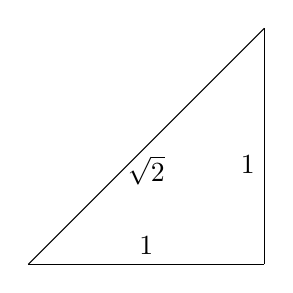
\begin{tikzpicture}[scale=3]
 \draw (0,0) -- node[above] {$1$} (1,0);
 \draw (1,0) -- node[below left] {$1$} (1,1);
 \draw (0,0) -- node[below] {$\sqrt{2}$}  (1,1);
 \end{tikzpicture} \end{center}
Annahme: \( \sqrt{2} \in \R\), aber \(\sqrt{2} \not\in \Q\)
\end{bsp}
\begin{proof} Angenommen $\displaystyle \sqrt{2} \in \Q$ \\
$ \displaystyle \sqrt{2} \in \Q \Rightarrow \frac{p}{q} \text{ mit }p \in \Z, q \in \N $ und p und q nicht beide durch 2 teilbar, sonst kürzen wir.
\begin{align*}
2 &= \frac{p^2}{q^2} &\Rightarrow\\
2q^2 &= p^2 &\Rightarrow &&\text{Also } 2 | p^2 \Rightarrow 2 | p \Rightarrow \exists m \text{ mit } p = 2 m. \\
2q^2 &= (2m)^2 = 4m^2 &\Rightarrow \\
q^2 &= 2m^2 & &&\text{ d.h. } 2 | q^2 \Rightarrow 2 | q \text{ Also p und q sind beide durch 2 teilbar.}
\end{align*}
 \WSP p und q sind nicht beide durch 2 teilbar. $\displaystyle \Rightarrow \sqrt{2} \not\in \Q \Rightarrow \sqrt{2} \in \R\setminus\Q$
\end{proof}

\begin{bem}
\( \sqrt{2} \) ist die positive Lösung von $ \displaystyle a^2 = 2 \Leftrightarrow a = \frac{2}{a} \Leftrightarrow  2a = a + \frac{2}{a} \Leftrightarrow a= \frac{1}{2}\left(a + \frac{2}{a}\right)$ \\
Betrachte die rechte Seite dieser Gleichung und berechne diese induktiv\\
Setze zB
\begin{align*}
a_1 &= 1\\
a_{n+1} &= \frac{1}{2}\left(a_n + \frac{2}{a_n}\right)
\end{align*}
\begin{align*}
a_1 = 1 && a_2 = 1,5 && a_3 \approx 1.41 && a_3 \approx 1,4142 &&\dots
\end{align*}
Also \(a_n\) nähert sich mit wachsendem \(n\) immer mehr an \(\sqrt{2}\). Dies führt zu dem Begriff \textbf{Grenzwert einer Folge}.
\end{bem}

\begin{defi}
Eine Folge $(a_n)_{k=0}^{\infty}$ reeller Zahlen ist eine Abbildung $\N_0 \rightarrow \R\text{ mit } n \mapsto a_n$
Bezeichnung: Wir schreiben für Folgen
\begin{align*}
&(a_n)_{k=0}^{\infty} && (a_n)_{n\ge0} && (a_n)_{n\in\N} & (a_n) && (a_n)_{n\ge n_0}
\end{align*}
\end{defi}

\newpage
\begin{defi}
Eine Folge \((a_n)\) heißt
\begin{enumerate}
\item (streng) monoton wachsend, wenn \( \fa a \in \N \sp a_n \le a_{n+1}	\quad (a_n)\nearrow	\quad (a_n < a_{n+1} \quad (a_n)\uparrow)\)
\item (streng) monoton fallend, wenn \( \fa a \in \N \sp a_n \ge a_{n+1}	\quad (a_n)\searrow	\quad (a_n > a_{n+1} \quad (a_n)\downarrow)\)
\item (streng) monoton, sie (streng) monoton wachsend oder (streng) monoton fallend ist.
\end{enumerate}
\end{defi}

\begin{bsp}
Ein paar Beispiele zu Folgen:
\begin{enumerate}[label=(\arabic*)]
\item Die konstante Folge \(a_n = k\) ist monoton fallend und steigend.
\item Die harmonische Folge $ \displaystyle a_n = \frac{1}{n} \sp \fa n \ge 1$ ist streng monoton fallend.
\item Die alternierende Folge $ \displaystyle a_n = (-1)^n $ ist nicht monoton.
\item Die geometische Folge $ \displaystyle  a_n = a^n \sp \fa n \ge 0 $ Sei $ \displaystyle a \in \R \sp a^n \text{ ist }
				\begin{cases}			\text{streng monoton wachsend} 	& a > 0\\
									\text{streng monoton fallend} 		& 0 < a < 1\\
									\text{monoton} 					& a = 1\\
									\text{nicht monoton} 				&  \end{cases} $
\item Die Fibonacci Folge ist monoton wachsend. $ \displaystyle f_n = \begin{cases}	1				& \text{wenn } n = 0, n = 1\\
																f_{n-1} + f_{n-2}	& \text{sonst} \end{cases} $
\end{enumerate}
\end{bsp}

\begin{defi}[Definition der Konvergenz]
Eine Folge reeller Zahlen \((a_n)_{n\in\N}\) heißt konvergent gegen \( a\in\R\) wenn
\[\forall \epsilon > 0 \spdot \exists N \in \N \spdot \forall n \ge N \spcolon \abs{a_n - a} < \epsilon\]
\(a\) heißt der Grenzwert oder Limes der Folge \((a_n)\). Die Folge \((a_n)\) heißt divergent, wenn sie nicht konvergiert. Schreibweise: \(\lim{a_n} = a \) oder \( \lim\limits_{n \to k}{a_n} = a \). Wobei \( k \in \R\cup\{\infty, -\infty\}\)
\end{defi}

\begin{bem}
Sei \(a \in \R, \epsilon > 0\). \(U_\epsilon(a) = (a-\epsilon, a+\epsilon) = \menge{x \in \R}{a - \epsilon < x < a + \epsilon} \text{ heißt } \epsilon\text{-Umgebung von }a\).
\[ a_n \in U_\epsilon(a) \Leftrightarrow a-\epsilon < a_n < a + \epsilon \Leftrightarrow -\epsilon < a_n - a < \epsilon \Leftrightarrow \abs{a_n - a} < \epsilon\]
Also: Die Folge \((a_n)\) konvergiert gegen \(a \Leftrightarrow \) Die Folgenglieder \(a_n\) liegen ab einer Schwelle \(N\) alle in der \(\epsilon\)-Umgebung von \(a\). \((a_n)\) konvergiert nicht gegen \(a \Leftrightarrow \exists \epsilon > 0 \spdot \forall N\in\N \spdot \exists n \ge N \spcolon \abs{a_n - a} \ge \epsilon\).
\end{bem}

\newpage
\begin{bsp}
Beispiele zur Konvergenz:
\begin{enumerate}[label=(\arabic*)]
	\item Die harmonische Folge konvergiert: $ \displaystyle a_n = \frac{1}{n} \Rightarrow \liminf{\frac{1}{n}} = 0$
	\begin{proof}
		Sei $ \displaystyle \epsilon > 0 \text{ und } N > \frac{1}{\epsilon} \qquad \abs{a_n - 0} = \abs{\frac{1}{n} - 0} = \frac{1}{n} \le \frac{1}{N} < \epsilon $
	\end{proof}
	\item Die alternierende Folge $ \displaystyle b_n = (-1)^n$ ist divergent
	\begin{proof}
		Angenommen $ \displaystyle \exists a \in \R \text{ mit } \liminf{b_n} = b \\
		\text{Wähle } \epsilon = \frac{1}{2} > 0 \Rightarrow \exists N \in \N \spdot \forall n \ge N \spcolon \abs{b_n - b} < \frac{1}{2} \text{. Da } b_{n+1} - b_n = 		\pm 2 \text{ ist } \forall n \ge N \\
		\vphantom{\frac{1}{2}}\ 2 = \abs{b_{n+1} - b_{n}} = \abs{b_{n+1} - b - (b_n - b)} \le \abs{b_{b+1} - b} + \abs{b_n - b} < \frac{1}{2} + \frac{1}{2} = 1 \Rightarrow 2 < 1 \\
		\WSP \Rightarrow (b_n) $ ist divergent.
	\end{proof}
	\item Ob die geometsiche Folge \((a^n)_{n\ge1}\) hängt davon ab, welchen Wert $a$ hat.
	\begin{proof} Durch Fallunterscheidung
		\begin{enumerate}
			\item[Fall 1:] \(\abs{a} < 1 \Rightarrow \liminf{a^n} = 0\) \\
				Sei \(\epsilon > 0 \overset{\text{Archimedisches Axiom}}{\Rightarrow} \sp \exists N \in \N \spcolon \abs{a}^N < \epsilon \Rightarrow \forall n \ge N \spcolon \abs{a^n - 0} = \abs{a}^n \le \abs{a}^N < \epsilon\)
			\item[Fall 2:] \(a =  1 \Rightarrow a^n = 1 \Rightarrow \lim{a^n} = 1\)
			\item[Fall 3:] \(a = -1 \Rightarrow \) divergent weil alternierend.
			\item[Fall 4:] \(\abs{a} > 1 \Rightarrow \forall K > 0 \spdot \exists n \in \N \spcolon \abs{a}^n > K \text{ , d.h. } (a^n)\) ist unbeschränkt.
		\end{enumerate}
	\end{proof}
\end{enumerate}
\end{bsp}

\begin{defi}
Eine Folge \((a_n)\) heißt nach oben (unten) beschränkt, wenn es ein \(A \in \R\) gibt mit \[\forall n \in \N \spcolon a_n \le A \quad \text{bzw.} \quad \forall n \in \N \spcolon a_n \ge A\]
\((a_n)\) heißt beschränkt, wenn \((a_n)\) nach oben oder unten beschränkt ist. d.h. \[\exists K \in \R \spdot \forall n \in \N \spcolon \abs{a_n} \le K \lor \abs{a_n} \ge K \]
\end{defi}

\begin{satz}
Jede konvergente Folge \((a_n)\) ist beschränkt.
\begin{proof}
\begin{math} \displaystyle
\begin{aligned}[t]
	&\liminf{a_n} = a. \quad \text{Wähle } \epsilon = 1 > 0 \Rightarrow \exists N \in \N \spdot \forall n \ge N \spcolon \abs{a_n - a} < 1 \\
	&\abs{a_n} = \abs{a + (a_n - a)} \le \abs{a} + \abs{a_n- a} < \abs{a} + 1 \quad \forall n \ge N \\
	&\text{Sei } K = max\{\abs{a_1}, \abs{a_2}, \dots, \abs{a_{n-1}}, \abs{a}+1\} \\
	&\abs{a_n} < K \quad \forall n \ge 1 \\
\end{aligned}
\end{math}
\end{proof}
\end{satz}

\begin{bem}
Die Umkehrung gilt nicht. Das heißt eine beschränkte Folge ist nicht konvergent.\\
\textit{Gegenbeispiel}: die alternierende Folge $(-1)^n$.
\end{bem}

\begin{satz}[Monotoniekriterium]
Sei $(a_n)$ eine Folge. Dann gilt:
\begin{itemize}
\item Ist $(a_n)$ monoton wachsend und nach oben beschränkt, dann ist $(a_n)$ konvergent.
\item Ist $(a_n)$ monoton fallend  und nach unten beschränkt, dann ist $(a_n)$ konvergent.
\end{itemize}
\begin{proof}
Es reicht die erste Aussage zu zeigen, denn ist $(a_n)$ monoton fallend und nach unten beschränkt \( \Rightarrow (-a_n)\) ist monoton wachsend und nach oben beschränkt $\Rightarrow (a_n) $ ist konvergent.\\
Sei also \((a_n) \nearrow \) und nach oben beschränkt. Mit dem Vollständigkeitsaxiom \(\Rightarrow \exists a = sup\menge{a_n}{n \in \N}\). Und sei $\epsilon > 0$
\begin{math}
\Rightarrow a - \epsilon \text{ ist keine obere Schranke von } \menge{a_n}{n \in \N} \Rightarrow \exists N \in \N \spcolon a-\epsilon < a_N \le a.\\
\text{Da }(a_n) \nearrow \begin{aligned}[t]
					&\Rightarrow \forall n \ge N 						&& a_N \le a_n \\
					&\Rightarrow a-\epsilon < a_N \le a_n \le a < a+\epsilon 	&& \forall n \ge N \\
					&\Rightarrow a-\epsilon < a_n < a+\epsilon 			&& \forall n \ge N \\
					&\Rightarrow \abs{a_n - a} < \epsilon					&& \forall n \ge N \\
					&\Rightarrow \liminf{a_n} = a \end{aligned}\end{math}
\end{proof}
\end{satz}

\begin{bem}
Das Monotonie-Kriterium ist äquivalent zur Vollständigkeit.
\end{bem}

\begin{satz}
Der Grenzwert einer Folge ist eindeutig bestimmt.
\begin{proof}
\begin{math} \displaystyle
\text{Angenommen } \liminf{a_n} = a\text{ und }\liminf{a_n} = b\text{ und } a \ne b.\\
\text{Sei }\epsilon = \frac{1}{2}\abs{b-a} \begin{aligned}[t]
								&\Rightarrow \exists N_1 \spdot \forall n \ge N_1 \spcolon \abs{a_n - a} < \epsilon \\
								&\Rightarrow \exists N_2 \spdot \forall n \ge N_2 \spcolon \abs{a_n - b} < \epsilon \end{aligned}\\
\text{Sei } N = max\{N_1, N_2\} \quad \forall n \ge N \spcolon
\begin{aligned}[t]
\abs{b-a} 	&= \abs{(b-a_n) + (a_n - a)} \\
		&\le \abs{b - a_n} + \abs{a_n - a} \\
		&= \abs{a_n - b} + \abs{a_n - a} \\
		&< \frac{1}{2}\abs{b-a} + \frac{1}{2}\abs{b-a} \\
		&= \abs{b-a}\\
\end{aligned}\\
\Rightarrow \abs{b-a}  < \abs{b-a} \WSP \Rightarrow a = b
\end{math}
\end{proof}
\end{satz}

\newpage
\begin{satz}[Rechenregeln für konvergente Folgen (RRF)]
Seien \((a_n)\) und \((b_n)\) zwei konvergente Folgen. Dann gilt:
\begin{enumerate}
\item \((a_n \pm b_n)\text{ ist konvergent und }\liminf{a_n  \pm  b_n} = \liminf{a_n}  \pm \liminf{b_n}\).
\item \(\lambda (a_n)\text{ ist konvergent und }\liminf{\lambda a_n} = \lambda \liminf{a_n}\).
\item \((a_n b_n)\text{ ist konvergent und }\liminf{a_n b_n} = \liminf{a_n} \lim{n}{b_n}\).
\item Ist $ \displaystyle (b_n) \ne 0 \sp \forall n \ge n_0\text{ und }\liminf{b_n} \ne 0\text{. Dann ist } \left(\frac{a_n}{b_n}\right) \text{ konvergent und }\liminf{\frac{a_n}{b_n}} = \frac{\liminf{a_n}}{\liminf{b_n}}$.
\item \(a_n \le b_n \text{ dann ist }\liminf{a_n} \le \liminf{b_n} \sp \forall n \ge n_0\).
\end{enumerate}
\begin{proof}
Sei \(\liminf{a_n} = 0\text{ und } \lim{b_n} = b\).
\begin{enumerate}
\item Sei $\epsilon > 0 \Rightarrow \exists N_1, N_2, \in \N \spcolon
\begin{aligned}[t]
&\abs{a_n - a} < \frac{\epsilon}{2} \quad \forall n \ge N_1 \quad \text{ und } \quad  \abs{b_n - b} < \frac{\epsilon}{2} \quad \forall n \ge N_2\\
&\Rightarrow \forall n \ge max\{N_1, N_2\}\\
& \begin{aligned}[t]
\abs{(a_n \pm b_n) - (a \pm b)} &= \abs{(a_n - a) \pm (b_n - b)} \\
&\le \abs{a_n - a} + \abs{b_n - b} < \frac{\epsilon}{2} + \frac{\epsilon}{2} = \epsilon.
\end{aligned}\\
&\Rightarrow (a_n \pm b_n) \text{ beschränkt und } \liminf{a_n \pm b_n} = a+b.
\end{aligned}$
\item Sei $ \displaystyle \epsilon > 0 \Rightarrow \exists N \in \N \begin{aligned}[t] \quad
		&\abs{a_n - a} < \frac{\epsilon}{\lambda} \quad \forall n \ge N\\
		& \abs{\lambda a_n - \lambda a} = \abs{\lambda(a_n - a)} = \abs{\lambda}\abs{a_n - a} < \lambda \frac{\epsilon}{\lambda} = \epsilon
		\end{aligned}$
\item Jede konvergente Folge ist beschränkt $ \displaystyle \Rightarrow \exists K \in \R \text{ mit } \abs{a_K} \le K \text{ und } \abs{b} \le K\vphantom{\frac{\epsilon}{2K}}\\
\text{Sei } \epsilon > 0 \Rightarrow \exists N_1, N_2 \in \N \spcolon \abs{a_n - a} < \frac{\epsilon}{2K} \text{ und } \abs{b_n - b} < \frac{\epsilon}{2K}. \Rightarrow \vphantom{\frac{\epsilon}{2K}} \\
\begin{aligned}[t]
\vphantom{\frac{\epsilon}{2K}} \forall n \ge max\{N_1, N_2\} \spcolon \abs{a_n b_n - a b} &= \abs{a_n b_n - a_n b + a_n b + a b} = \abs{ a_n (b_n - b) + b (a_n - a)} \\
&\le \abs{ a_n (b_n - b)} + \abs{b (a_n - a)} \\
&= \underbrace{\abs{a_n}}_{\le K} \abs{b_n - b} + \underbrace{\abs{b}}_{\le K}\abs{a_n - a} < K \frac{\epsilon}{2K} + K \frac{\epsilon}{2K} = \epsilon
\end{aligned}$
\item
Zeige \begin{math} \displaystyle \liminf{\frac{1}{b_n}} = \frac{1}{\liminf{b_n}} \quad\Rightarrow  \abs{\abs{ b_n } - \abs{b}} \le \abs{ b_n - b} < \frac{\abs{b}}{2} \quad \forall n \ge n_0 \\
\Rightarrow -\frac{\abs{b}}{2} < \abs{b_n} - \abs{b} < \frac{\abs{b}}{2} \Rightarrow  \frac{\abs{b}}{2} < \abs{b_n} \quad \Rightarrow \frac{1}{\abs{b_n}} < \frac{2}{\abs{b}} \quad \forall n \ge n_0 \\
\text{Sei } \epsilon > 0 \Rightarrow \exists N \quad \forall n \ge N \quad \abs{b_n - b} < \frac{\epsilon \abs{b} ^2}{2} \Rightarrow \\
\abs{\frac{1}{b_n} - \frac{1}{b}} = \abs{\frac{b - b_n}{b b_n}} = \frac{1}{\abs{b_n}}\frac{1}{\abs{b}} \abs{b - b_n} < \frac{2}{\abs{b}}\frac{1}{\abs{b}}\abs{b_n - b} < \frac{2}{\abs{b}^2}\frac{\epsilon\abs{b}^2}{2} = \epsilon.
\end{math}
\item Sei \(a_n \le b_n \quad \forall n \ge n_0. \) \quad Angenommen \(a > b\). \quad Sei \begin{math} \displaystyle \epsilon =  \frac{a-b}{2} > 0 \\
\Rightarrow \exists N_1, N_2 \in \N \spcolon \abs{a_n - a} < \epsilon \quad \forall n \ge N_1 \qquad \text{und} \qquad \abs{b_n - b} < \epsilon \quad \forall n \ge N_2 \vphantom{\frac{a-b}{2}} \\
\begin{aligned}[t]
b_n < b + \epsilon &= b + \frac{a-b}{2} = \frac{2b + a - b}{2} = \frac{b + a}{2} = \frac{2a - a + b}{2} \\
&= a - \frac{a-b}{2} = a - \epsilon < a_n && \quad \forall n \ge max\{N_1, N_2\}
\end{aligned} \\
\Rightarrow  b_n < a_n \quad \forall n \ge max\{N_1, N_2\} \quad \WSP \Rightarrow a \le b
\end{math}
\end{enumerate}
\end{proof}
\end{satz}

\begin{satz}[Sandwich-Theorem]
Sei \((a_n)\text{ und }(b_n)\) zwei konvergente Folgen mit der Eigenschaft, dass \(\liminf{a_n} = \liminf{b_n} = a\).
Sei \((c_n)\) eine Folge mit der Eigenschaft, dass \(a_n \le c_n \le b_n \quad \forall n \ge n_0\).
Dann ist \((c_n)\) konvergent und \(\liminf{c_n} = a\).
\begin{proof}
\begin{math}
\begin{aligned}[t] \displaystyle \text{Sei }\epsilon > 0 &\Rightarrow \exists  N_1, N_2 \in \N \quad
&&\begin{aligned}[t] a - \epsilon < a_n < a + \epsilon & \quad \forall n \ge N_1 \\
			   a - \epsilon < b_n < a + \epsilon & \quad \forall n \ge N_2
\end{aligned} \\
&\Rightarrow \forall n \ge max\{N_1, N_2\} \sp \text{gilt: } \quad &&\begin{aligned}[t] &a-\epsilon < a_n \le c_n \le b_n < a + \epsilon \quad  \forall n \ge N \\
&\Rightarrow \abs{c_n - a} < \epsilon \Rightarrow \liminf{c_n} = a
\end{aligned}
\end{aligned}\\
\end{math}
\end{proof}
\end{satz}

\begin{bsp}
Zwei Beispiele zum Sandwich-Theorem:
\begin{enumerate}
\item Sei \((a_n)\) eine Folge mit \(0 \le a_n \le \frac{1}{n} \Rightarrow \liminf{a_n} = 0\)
\item \(a_n = \sqrt{2n} - \sqrt{n}\) ist divergent, denn \\
$ \displaystyle a_n = \frac{\left(\sqrt{2n} - \sqrt{n}\right)\left(\sqrt{2n} + \sqrt{n}\right)}{\left(\sqrt{2n} + \sqrt{n}\right)} = \frac{2n - n}{\sqrt{n} \underbrace{\left(\sqrt{2} - 1\right)}_{\le3}} \ge \frac{n}{3\sqrt{n}} = \frac{\sqrt{n}}{3} \ge \sqrt{n} \longtoinf \infty $.
\end{enumerate}
\end{bsp}

\begin{defi}
Eine Folge \((a_n)\) heißt bestimmt divergent gegen \(\pm \infty \) wenn gilt:
\[\forall K \in \R \spdot \exists N \in \N \spdot \forall n \ge N \spcolon  a_n \lessgtr K \]
Für jedes $K$ aus \R  gibt es ein $N$ aus \N ab dem $a_n$ größer/kleiner als $K$ wird. Schreibweise: \(\liminf{a_n} = \pm \infty \)
\end{defi}

\begin{bsp}
Beispiele zu bestimmt divergenten Folgen:
\begin{enumerate}
\item Die Fibonacci Folge ist bestimmt divergent gegen \(+ \infty = \infty \)
\item Sei \(a_n = n\text{, dann folgt }\liminf{a_n} = \infty\)
\item Sei \(\liminf{a_n} = \infty \Leftrightarrow \liminf{-a_n} = - \infty\)
\item Die Folge \(a_n = (-1)^n\) ist divergent aber nicht bestimmt divergent.
\item Sei \((a_n)\) bestimmt divergent und $ \displaystyle a_n \ne 0 \quad \forall n \ge n_0\text{, dann folgt }\liminf{\frac{1}{a_n}} = 0$.
\begin{proof}Sei $ \displaystyle \liminf{a_n} = \infty \quad
\begin{aligned}[t] &&\forall \epsilon > 0 \spdot \exists N \in \N \spdot \forall n \ge N \spcolon a_n &> \frac{1}{\epsilon} > 0 \\
&&\Rightarrow \frac{1}{a_n} &< \epsilon \Rightarrow \abs{\frac{1}{a_n} - 0} < \epsilon  \\
&&\text{da } a_n > 0 \Rightarrow \liminf{\frac{1}{a_n}} = 0.
\end{aligned}$\\
\end{proof}
\end{enumerate}
\end{bsp}

\begin{defi}
Sei \((a_n)\) eine Folge reeller Zahlen und \(n_0 < n_1 < n_2 < \dots < n_k < \dots \) eine Teilmenge von \N.\\
Dann heißt die Folge \((a_{n_k})_{k \in \N }\) eine Teilfolge von \((a_n)_{n \in \N}\).
\end{defi}

\begin{bem}
Ist die Folge \((a_n)\) konvergent, dann ist auch jede Teilfolge von \((a_n)\) konvergent.
\begin{proof} Sei $(a_n)$ konvergent gegen $a$. Also $ \forall \epsilon > 0 \spdot \exists N \in \N \spcolon \abs{a_n - a} < \epsilon \quad \forall n \ge N$. Da $(a_{n_k})$ eine Teilfolge von $(a_n)$ mit $n_0 < n_1 < n_2 < \dots < n_k < \dots$ und da $n_k$ monoton steigend ist, ist $k \le n_k$ und $n_k \ge N \quad \forall k \ge N $ daraus folgt $\abs{a_{n_k} - a} < \epsilon \quad \forall n \ge N$.
\end{proof}
\end{bem}

\begin{defi}
Sei \((a_n)\) eine Folge. Eine Zahl \(a \in \R\) heißt Häufungspunkt (Häufungswert) der Folge \((a_n)\), wenn es eine Teilfolge von \((a_n)\) gibt, die gegen \(a\) konvergiert.
\end{defi}

\begin{bem}
Beispiele zu Häufungspunkten:
\begin{enumerate}
\item Sei \(\liminf{a_n} = a\), dann ist \(a\) der einzige Häufungspunkt der Folge \((a_n)\).
\item Eine bestimmt divergente Folge hat keinen Häufungspunkt.
\item Die Folge $ \displaystyle a_n = \frac{1}{n}+ (-1)^n $ besitzt die zwei Häufungspunkte $ \displaystyle \pm 1:\\
\begin{aligned}[t] &\liminf{a_{2n}} &&= \liminf{\frac{1}{2n} (-1)^{2n}} &&= \liminf{\frac{1}{2n}} + 1 &&= 1 \\
&\liminf{a_{2n+1}} &&= \liminf{\frac{1}{2n+1} (-1)^{2n+1}} &&= \liminf{\frac{1}{2n+1}} - 1 &&= - 1
\end{aligned}$
\item Jede konvergente Folge ist beschränkt, aber jede beschränkte Folge muss nicht konvergent sein.
\end{enumerate}
\end{bem}

\begin{satz}[Satz von Bolzano-Weierstraß]
Jede beschränkte Folge reeller Zahlen besitzt eine konvergente Teilfolge.
\begin{proof}
\begin{math} \displaystyle
\begin{aligned}[t]
&(a_n)_{n \in \N_0} \text{ ist beschränkt, d.h. }\exists A \in \R \text{ mit }-A \le a_n \le A \quad \forall n \ge 0\\
&\text{Sei } A_k = \menge{a_m}{m \ge k} \text{. Beachte: dass jede der Mengen } A_k \text{ beschränkt ist, durch }A\\
&\text{Daraus folgt mit dem Vollständigkeitsaxiom } \exists \sp inf(A_k) \quad \forall A_k \qquad \text{Wähle } x_k = inf(A_k). \\
&\text{Da } A_0 \supset A_1 \supset \dots \supset A_k \supset A_{k+1} \supset \dots \quad \Rightarrow \quad x_k \le x_{k+1} \quad \forall k \ge 0.\\
&\text{Betrachte die Folge }(x_n)_{k \ge 0}. \quad (x_n) \text{ ist monoton wachsend und durch $A$ beschränkt.}\\
&\text{Mit dem Monotoniekritierium konvergiert } (x_n). \quad \text{Sei etwa } \liminf[k]{x_k} = z\\
&\zz z \text{ ist Häufungspunkt von } (a_n) \\
&\begin{aligned}[t]
& 1. &&\text{Sei } \epsilon > 0 \text{ , da } \liminf[k]{x_k} = z \Rightarrow \exists N \in \N \text{ mit } \abs{x_k - z} < \frac{\epsilon}{2} \quad \forall n \ge N \\
& 2. &&\text{Da }x_k = inf(A_k) = inf\menge{a_m}{m \ge k} \Rightarrow \exists a_{k_m} \text{ mit } \abs{x_k - a_{k_m}} < \frac{\epsilon}{2}.
\end{aligned} \\ \vphantom{\frac{\epsilon}{2}}
&\qquad \Rightarrow \abs{a_{k_m} - z} = \abs{a_{k_m} - x_k + x_k - z} \le \abs{a_{k_m} - x_k} + \abs{x_k - z} < \frac{\epsilon}{2} + \frac{\epsilon}{2} = \epsilon  \\ \vphantom{\frac{\epsilon}{2}}
&\qquad \text{Also } \forall \epsilon > 0 \spdot \exists N \in \N \spdot \forall k \ge N \spdot \exists a_{k_m} \in (a_n) \spcolon \abs{a_{k_m} - z} < \epsilon  \\
&\qquad \text{d.h. die Teilfolge }(a_{k_m})_{m\ge 0}\text{ ist konvergent gegen } z \\
&\text{Also }(a_{k_m})\text{ ist eine konvergente Teilfloge von der beschränkten Folge }(a_n).
\end{aligned} \\
\end{math}
\begin{figure}[h!] \begin{center} 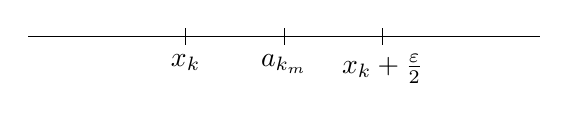
\begin{tikzpicture}
    \draw(-1,0)--(5.5,0);
    \foreach \x/\xtext in {1/{x_k},2.25/{a_{k_m}},3.5/{x_k + \frac{\epsilon}{2}}}
      \draw(\x,3pt)--(\x,-3pt) node[below] {$\xtext$};
\end{tikzpicture} \end{center}\end{figure}
\end{proof}
\end{satz}

\begin{bem}
Der Satz von Bolzano-Weierstraß ist äquivalent zum Vollständigkeitsaxiom. Andere äquivalente Formulierungen zu Bolzano-Weierstraß:
\begin{itemize}
\item Jede beschränkte Folge reeller Zahlen hat mindestens einen Häufungspunkt.
\item Jede beschränkte Folge reeller Zahlen hat einen größten und einen kleinsten Häufungspunkt.
\end{itemize}
\end{bem}

\begin{defi}[Definition einer Cauchy-Folge]
Eine Folge \((a_n)_{n \ge 0}\) heißt CAUCHY-Folge, wenn gilt:
\[\forall \epsilon > 0 \spdot \exists N \in \N \spdot \forall n, m \ge N \spcolon \abs{a_n - a_m} < \epsilon\]
\end{defi}

\begin{satz}
Folgende Aussagen sind äquivalent
\begin{enumerate}
\item Die Folge \((a_n)\) ist konvergent
\item Die Folge \((a_n)\) ist eine Cauchy-Folge
\end{enumerate}
\begin{proof}
\begin{math} \displaystyle
\begin{aligned}[t]
1) \Rightarrow 2) \quad &\text{Sei }\liminf{a_n} = a \Rightarrow \forall \epsilon > 0 \spdot \exists N \spdot \forall m \ge N \spcolon \abs{a_n - a} < \frac{\epsilon}{2} \\
&\Rightarrow \forall n, m \ge N \spcolon \abs{a_n - a_m} = \abs{a_n - a + a - a_m} \le \underbrace{\abs{a_n - a }}_{<\frac{\epsilon}{2}}  + \underbrace{\abs{a_m - a}}_{<\frac{\epsilon}{2}} < \epsilon \\
&\Rightarrow a_n \text{ ist eine Cauchy Folge}\\
2) \Rightarrow 1) \quad &\text{Jede Cauchy Folge ist beschränkt.} \\
& \text{Sei } \epsilon = 1 \Rightarrow \exists N \in \N \spdot \forall n, m \ge N \spcolon \abs{a_n - a_m} < 1 \quad \Rightarrow \abs{a_n - a_N} < 1 \\
&\Rightarrow \abs{a_n} = \abs{a_n - a_N + a_N} \le \abs{a_n - a_N} + \abs{a_N} < 1 + \abs{a_N} \quad \forall n  \ge N\\
&\Rightarrow \forall n \in \N \spcolon \abs{a_n} \le max\{\abs{a_0},\dots,\abs{a_{N-1}},\abs{a_N} + 1\} \Rightarrow (a_n) \text{ ist beschränkt.}\\
&\text{Nach Bolzano-Weierstraß existiert eine konvergente Teilfolge: } (a_{n_k}) \longtoinf[k] a\\
&\zz \liminf{a_n} = a.\\
&\text{Sei }\epsilon > 0. \text{ Wähle $m$ so groß, dass }\begin{aligned}[t]&\abs{a_m - a_n} < \frac{\epsilon}{2} \quad \forall n,m \ge N \text{ und } \\
&\abs{a_{n_k} - a} < \frac{\epsilon}{2} \quad \forall n_k \ge k \ge N \end{aligned} \\
&\Rightarrow \abs{a-a_n} = \abs{a - a_{n_k} + a_{n_k} - a_n} \le \abs{a- a_{n_k}} + \abs{a_{n_k} - a_n} < \frac{\epsilon}{2} + \frac{\epsilon}{2} = \epsilon
\end{aligned}\\
\end{math}
\end{proof}
\end{satz}

\begin{bsp}[Verfahren zur Berechnung der Quadratwurzel]
Seien \(a = 0\), \(a_0 > 0\) reelle Zahlen. Wir definieren die Folge \((x_n)\) rekursiv.
\begin{align*}
x_0 &= x_0 \\
x_{n+1} &= \frac{1}{2}\left(x_n + \frac{a}{x_n}\right)
\end{align*}
Wir zeigen: \((x_n)\) ist konvergent und \(\liminf{x_n} = x \text{ und } x^2 = a\).
\begin{proof}$\begin{aligned}[t]
&\zz \begin{aligned}[t] &\text{nach unten durch $0$ beschränkt: } x_n > 0 \quad \forall n \ge 0 \\
&\IA \quad  x_0 > 0 \\
&\IV x_{n+1} = \frac{1}{2}\left(x_n + \frac{a}{x_n}\right) \\
&\IS \\
&\text{Sei } x_n > 0 \Rightarrow x_{n+1} = \underbrace{\frac{1}{2}}_{> 0}\bigg( \underbrace{x_n}_{> 0} + \underbrace{\overbrace{\frac{a}{x_n}}^{> 0}}_{>0}\bigg) > 0 \Rightarrow (x_n) \text{ ist n.u. durch $0$ beschränkt.} \end{aligned} \\
&\zz \begin{aligned}[t] &x_n^2 \ge a \quad \forall n \ge 1 \text{ denn } \\
&x_{n+1}^2 - a \begin{aligned}[t] &= \frac{1}{4}\left(x_n + \frac{a}{x_n}\right)^2  - a = \frac{1}{4}\left(x_n^2 + 2x_n\frac{a}{x_n} + \frac{a^2}{x_n^2} \right) - a \\
&= \frac{1}{4}\left(x_n^2 + \frac{2ax_n}{x_n} + \frac{a^2}{x_n^2} - 4a \right) = \frac{1}{4} \left(x_n^2 + \frac{2ax_n}{x_n} + \frac{a^2}{x_n^2} -\frac{4ax_n}{x_n} \right)\\
&= \frac{1}{4} \left(x_n^2 - 2x_n\frac{a}{x_n} + \frac{a^2}{x_n^2} \right) = \frac{1}{4} \left(x_n - \frac{a}{x_n} \right)^2 \ge 0
\end{aligned}
\end{aligned} \\
&(x_n)\text{ ist monoton fallend} \\
&x_n - x_{n+1} = x_n - \frac{1}{2} \left(x_n + \frac{a}{x_n}\right) =\frac{1}{2} \left(2x_n - x_n - \frac{a}{x_n}\right) = \frac{1}{2x_n\underbrace{(x_n^2 - a)}_{x_n^2 > a}} \ge 0 \\
&\Rightarrow x_n \ge x_{n+1} \\
&\text{Nach dem Monotonie-Kriterium ist $(x_n)$ konvergent.} \\
&\text{Sei } x= \liminf{x_n} \quad \begin{aligned}[t] x &= \liminf{x_{n+1}} = \liminf{\frac{1}{2}\left(x_n + \frac{a}{x_n}\right)} \\
&= \frac{1}{2}\left(\liminf{x_n} + \frac{a}{\liminf{x_n}}\right) =  \frac{1}{2}\left(x + \frac{a}{x}\right)
 \end{aligned} \\
&\Rightarrow 2x = x + \frac{a}{x} \quad \Rightarrow x = \frac{a}{x} \quad \Rightarrow x^2 = a
\end{aligned}\\$
\end{proof}
Die positive Lösung der Gleichung \(x^2 = a\) heißt die Quadratwurzeln von \(a\). Wir schreiben \(x = \sqrt{a}\).
\end{bsp}

\newpage
\section{Reihen}

\begin{defi}
Sei \((a_n)_{n \ge 0}\) eine Folge reeller Zahlen. Sei weiters $ \displaystyle S_N = \sum_{n = 0}^{N}{a_n} $ die $N$-te Partialsumme, dann heißt die Folge \((S_N)_{N \ge 0}\) der Partialsummen eine unendliche Reihe.
\[ \text{Schreibweise: }\suminf{a_n} \]
Konvergiert die Folge \((S_N)\text{ mit }\liminf{S_N} = s \text{, dann heißt } \suminf{a_n} = s\) der Wert der Reihe. Man sagt: Die Reihe \(\suminf{a_n}\) konvergiert.
\[ \text{Schreibweise: } \suminf{a_n} < \infty \]
\end{defi}

\begin{bsp}\
\begin{enumerate}
\item Die geometrische Reihe:
\begin{math}\displaystyle \begin{aligned}[t]
&\suminf{a^n} = \frac{1}{1-a} \text{ , wenn } \abs{a} < 1 \\
&\suminf{a^n} \text{ ist divergent, wenn } \abs{a} \ge 1
\end{aligned}\end{math} 

\begin{proof}
\begin{math}\displaystyle \begin{aligned}[t]
&\IA[N=0] \quad a^0 = \frac{(1-a)}{(1- a)} = 1 \\
&\IV \sum_{n = 0}^{N}{a^n} = \frac{1-a^{N+1}}{1-a} \\
&\IS[N \mapsto N+1] \\
&\sum_{n = 0}^{N+1}{a^n} = a^{N+1} + \sum_{n = 0}^{N}{a^n} \overset{IV}{=} a^{N+1} + \frac{1-a^{N+1}}{1-a} = \text{... selber} \\ %TODO
&\text{Sei }S_N = \sum_{n=0}^{N}{a^n} = \frac{1 - a^{N+1}}{1- a} \\
&\text{Sei }\abs{a} < 1\text{. Dann folgt }\liminf{a^N} = 0 \\
&\Rightarrow \liminf{S_N} = \liminf{\frac{1-a^{N+1}}{1-a}} = \frac{1}{1-a} \\
&\text{Sei }a \ge 1 \Rightarrow \sum_{n=0}^{N}{a^n} \ge \sum_{n=0}^{N}{1} = N+1 \longrightarrow \inf \\
&\text{Sei }a \le -1 \Rightarrow a = -b \text{ mit }b \ge 1 \Rightarrow \sum_{n=0}^{N}{a^n} \ge \sum_{n=0}^{N}{(-1)^nb^n} \text{ divergent}
\end{aligned}\end{math} 
\end{proof}

\item Die harmonische Reihe:
\[\sum_{n=1}^{\infty}{\frac{1}{n}} = +\infty\]

\begin{proof}
\begin{math}\displaystyle \begin{aligned}[t]
&S_{2^N} = \sum_{n = 1}^{2^N}{\frac{1}{n}} =
1 +\underbrace{\frac{1}{2}}_{=\frac{1}{2}} + \underbrace{\frac{1}{3} + \frac{1}{4}}_{=\frac{1}{2}} + \underbrace{\frac{1}{5} + \frac{1}{6} + \frac{1}{7} + \frac{1}{8}}_{=\frac{1}{2}} +  ... + \underbrace{\frac{1}{2^{N-1}+1}+ .... + \frac{1}{2^N}}_{=\frac{1}{2}} \\
&\ge 1 + n \frac{1}{2} > \frac{n}{2} \longrightarrow +\infty
\end{aligned}\end{math} 

Würde \((S_N)_{N\ge1}\) konvergieren, dann auch die Teilfolge \((S_{2^N})_{N \ge 1}\), da diese dievergiert, divergiert auch \((S_N)_N\)\\
\end{proof}

\item
\[ \Suminf{\frac{1}{n(n+1)}}= 1 \]

\begin{proof}
\begin{math}\displaystyle \begin{aligned}[t]
&S_N = \sum_{n=1}^{N}{\frac{1}{n(n+1)}} = \sum_{n=1}^{N}{\frac{1}{n}} - \frac{1}{n+1} = \sum_{n=1}^{N}{\frac{1}{n}} - \sum_{n=1}^{N}{\frac{1}{n+1}}
= 1 + \sum_{n=2}^{N}{\frac{1}{n}} - \sum_{n=2}^{N+1}{\frac{1}{n}} \\
&= 1 + \sum_{n=2}^{N}{\frac{1}{n}} - \sum_{n=2}^{N}{\frac{1}{n}} + \frac{1}{N+1}
= 1 + \frac{1}{N+1} \longrightarrow 1
\end{aligned}\end{math} 
\end{proof}

\end{enumerate}
\end{bsp}

\begin{satz}
Seien \suminf{a_n} und \suminf{b_n} zwei konvergente Reihen und \(\lambda \in \R\),
dann ist auch \(\suminf{\lambda a_n + b_n}\) konvergent und \(\suminf{\lambda a_n + b_n} = \lambda \suminf{a_n} + \suminf{b_n}\)
\begin{proof}
folgt auf Grund der Rechenregeln für konvergente Folgen.
\end{proof}
\end{satz}

\begin{satz}[Cauchy-Kriterium für Reihen]
Die Reihe \(\suminf[k]{a_k}\) ist konvergent, genau dann wenn gilt:
% TODO Florian
\[\forall \epsilon > 0 \spdot \exists N(\epsilon) \in \N \spdot \forall n \ge m \ge N \spcolon \abs{\sum_{k=m}^{n}{a_k}} < \epsilon \qquad (\star)\]
\((\star)\) bedeutet die \((S_n)_n\) ist eine Cauchy-Folge \(\Leftrightarrow (S_n)_n\) ist konvergent
\begin{proof}
\(S_n - S_m = \sum_{k=0}^{n}{a_k} - \sum_{k=0}^{m}{a_k} = \sum_{k=m}^{n}{a_k}\).\\
\end{proof}
\end{satz}

\begin{korr}
Ist \suminf[k]{a_k} konvergent \(\Rightarrow \liminf[k]{a_k} = 0\).
\begin{proof}
\begin{math}\displaystyle \begin{aligned}[t]
&\text{Sei } a_n = \sum_{k = m}^{n}{a_k}, \text{ da } \suminf[k]{a_k} < \infty \text{ folgt mit dem Cauchy-Kriterium }\\
&\forall \epsilon > 0 \spdot \exists N \in \N \spdot \forall n \ge N \spcolon \abs{a_N} = \abs{ \sum_{k = m}^{n}{a_k}} < \epsilon \Rightarrow \liminf{a_n} = 0\\
\end{aligned}\end{math} 
\end{proof}
\end{korr}

\begin{bem}
Die Umkehrung des Korrolars gilt nicht. z.B. \(\liminf{\frac{1}{n}} = 0 \text{ aber } \suminf{\frac{1}{n}} = \infty \) (harmonische Reihe).
\end{bem}

\begin{defi}
Die Reihe \suminf[k]{a_k} heißt absolut konvergent, wenn die Reihe \suminf[k]{\abs{a_k}} konvergiert.
\end{defi}

\begin{satz}
Jede absolut konvergente Reihe ist auch konvergent.
\begin{proof}
\begin{math}\displaystyle \begin{aligned}[t]
&\text{Sei }\suminf[k]{\abs{a_k}} < \infty  \overset{\text{Cauchy-Kriterium}}{\Rightarrow} \forall \epsilon > 0 \spdot \exists N \in \N \spdot \forall n \ge m \ge N \spcolon \abs{\sum_{k=m}^{n}{\abs{a_k}}} < \epsilon \\
&\overset{\text{Dreiecksungleichung}}{\Rightarrow} \abs{\sum_{k=m}^{n}{a_k}} \le \abs{\sum_{k=m}^{n}{\abs{a_k}}} < \epsilon \text{ gilt } \forall n \ge m \ge N \\
&\text{mit dem Cauchy-Kriterium folgt } \suminf[k]{a_k}\text{ ist konvergent.}
\end{aligned}\end{math} 
\end{proof}
\end{satz}

\begin{bem}
Die Umkehrung des Satzes gilt nicht. zB kann man zeigen, dass die Reihe \(\suminf[k]{(-1)^k\frac{1}{k}}\) konvergiert. Aber die Reihe \(\suminf[k]{\abs{(-1)^k\frac{1}{k}}} = \suminf[k]{\frac{1}{k}} = \infty\)
\end{bem}

\begin{satz}[Majoranten-Kriterium]
\begin{math}\displaystyle \begin{aligned}[t]
&\text{Sei } \suminf[k]{b_k} \text{ konvergent mit } b_k \ge 0 , \forall k \ge N_0 \\
&\text{Sei } (a_k)_{k=0}^{\infty} \text{ eine Folge mit } \abs{a_k} \le b_k , \forall k \ge N_0 \\
&\Rightarrow \suminf[k]{a_k} \text{ ist absolut konvergent.}
\end{aligned}\end{math}

\begin{proof}
\begin{math}\displaystyle \begin{aligned}[t]
&\text{Sei } \suminf[k]{b_k} < \infty \text{ und } b_k > 0 \\
&\overset{\text{Cauchy-Kriterium}}{\Rightarrow} \forall \epsilon > 0 \spdot \exists N \in \N \spdot \forall n \ge m \ge N \spcolon \abs{\sum{k=m}{n}{b_k}} < \epsilon \\
&\overset{\abs{a_k} \le b_k}{\Rightarrow} \abs{\sum{k=m}{n}{\abs{a_k}}} \le \abs{\sum{k=m}{n}{b_k}} < \epsilon \text{ gilt } \forall n \ge m \ge N \\
&\overset{\text{Cauchy-Kriterium}}{\Rightarrow} \suminf[k]{\abs{a_k}} \text{ ist konvergent} \\
&\Rightarrow \suminf[k]{a_k}\text{ ist absolut konvergent.}
\end{aligned}\\\end{math} 
\end{proof}
\end{satz}

\begin{korr}[Minoranten-Kriterium]
\begin{math}\displaystyle \begin{aligned}[t]
\hphantom{mmmm}\\
&\text{Sei } \suminf[k]{b_k} \text{ divergent mit } b_k \ge 0 , \forall k \ge N_0 \\
&\text{Sei } (a_k)_{k=0}^{\infty} \text{eine Folge mit } \abs{a_k} \ge b_k , \forall k \ge N_0 \\
&\Rightarrow \suminf[k]{a_k} \text{ ist auch divergent.}
\end{aligned}\end{math}

\begin{proof}
Wäre $\displaystyle\suminf[k]{a_k}$ konvergent, dann wäre nach dem Majoranten-Kriterium $\displaystyle \suminf[k]{b_k}$ konvergent, da $\displaystyle \abs{b_k} \le a_k$. \WSP
\end{proof}
\end{korr}

\begin{satz}[Quotienten-Kriterium]
\begin{math}\displaystyle \begin{aligned}[t]
&\text{Sei } \suminf{a_n} \text{ eine Reihe mit } a_n \ne 0 , \forall n \ge n_0 \\
&\exists q\in \R \text{ mit } 0 < q < 1 \text{, sodass } \abs{\frac{a_{n+1}}{a_n}} \le q < 1, \forall n \ge n_0 \Rightarrow \suminf{a_n} \text{ ist absolut konvergent.}
\end{aligned}\end{math}

\begin{proof}
\begin{math}\displaystyle \begin{aligned}[t]
&\text{Sei } \abs{\frac{a_{n+1}}{a_n}} \le q < 1 \quad \forall n \ge 0 \text{ (o.B.d.A.)} \Rightarrow \abs{a_{n+1}} \le q \abs{a_n} \\
&\Rightarrow \abs{a_n} \le q\abs{a_{n-1}} \le q^2 \abs{a_{n-2}} \le ... \le q^n \abs{a_0} \text{Also } \abs{a_n} \le q^n \abs{a_0}\\
&\text{Da } \suminf{\abs{a_n}} \le \suminf{q^n \abs{a_0}} = \abs{a_0} \suminf{q^n} = \abs{a_0} \frac{1}{1-q} \text{, da } 0 < q < 1 \text{ (geometrische Reihe)} \\
&\text{mit dem Majoranten-Kriterium folgt } \suminf{a_n} \text{ ist absolut konvergent.}
\end{aligned}\\\end{math}
\end{proof}
\end{satz}

\begin{korr}[einfaches Quotienten-Kriterium]
\begin{math}\displaystyle \begin{aligned}[t]
&\text{Sei } a_n \ne 0 \sp \fa n > n_0 \text{ und existiert } \liminf{\abs{\frac{a_n+1}{a_n}}} \text{ und ist } \liminf{\abs{\frac{a_n+1}{a_n}}} < 1 \\
&\Rightarrow \suminf{a_n} \text{ ist absolut konvergent.}
\end{aligned}\end{math} 

\begin{proof}
\begin{math}\displaystyle \begin{aligned}[t]
&\text{Sei } \liminf{\abs{\frac{a_n+1}{a_n}}} = \alpha < 1 \\
&\text{Sei } \epsilon = \frac{1 - \alpha}{2} > 0 \\
&\Rightarrow \exists N \spdot \forall n \ge N \spcolon \abs{\abs{\frac{a_{n+1}}{a_n}} - \alpha} < \epsilon  = \frac{1-\alpha}{2} \\
&\Rightarrow \abs{\frac{a_{n+1}}{a_n}} < \frac{1-\alpha}{2} + \alpha = \frac{1+\alpha}{2} \overset{\text{da } \alpha < 1}{<} \frac{1+1}{2} = 1 \\
&\text{Setze } q = \frac{1 + \alpha}{2} < 1 \text{ und } \abs{\frac{a_{n+1}}{a_n}} < q < 1 \\
&\text{mit dem Quotienten-Kriterium folgt }\suminf{a_n} \text{ ist absolut konvergent.}
\end{aligned}\\\end{math} 
\end{proof}
\end{korr}

\begin{bsp}
Einige Beispiele zur Konvergenz von Reihen.
\begin{enumerate}
\item % TODO 1. is not properly aligned
\begin{math}\displaystyle \begin{aligned}[t]
&\suminf{\frac{1}{n^k}} < \infty \qquad \forall k \ge 2 \\
&\text{[Bemerkung: Die Konvergenz gilt auch \(\fa k \in \R, k > 1\) ohne Beweis]}
\end{aligned}\end{math} 

\begin{proof}
\begin{math}\displaystyle \begin{aligned}[t]
&\frac{1}{n^k} \le \frac{1}{n^2} \quad \forall k \ge 2 \\
&\text{ und } \frac{1}{n^2} \le \frac{2}{n(n+1)} \text{ , denn } 2n^2 \ge n(n+1) \Leftrightarrow n^2 \ge n \Leftrightarrow n \ge 1 \\
&\Rightarrow \frac{1}{n^k} \le \frac{2}{n(n+1)} \quad \forall k \ge 2 \\
&\text{ und } \suminf{\frac{2}{n(n+1)}} = 2 \suminf{\frac{1}{n(n+1)}} = 2 \cdot 1 = 2 \\
&\overset{Majoranten-Kriterium}{\Rightarrow} \suminf{\frac{1}{n^k}} < \infty \quad \forall k \ge 2
\end{aligned}\\\end{math} 
\end{proof}
Frage: Wie sind die Werte der Reihe $\displaystyle \suminf{\frac{1}{n^k}} \text{ für } k \ge 2 $ ? \\
Euler: $ \displaystyle \suminf{\frac{1}{n^2}} = \frac{\pi^2}{6} \text{ , } \suminf{\frac{1}{n^4}} = \frac{\pi^4}{90} \text{ , \dots , } \suminf{\frac{1}{n^{2k}}} = C_k \pi^{2k}$ \\
Aber: $\displaystyle \suminf{\frac{1}{n^3}} \in \R \setminus \Q \text{ , } \suminf{\frac{1}{n^5}} = \text{? } \text{, \dots , } \suminf{\frac{1}{n^{2k+1}}} = \text{? }$

\item
$\displaystyle \text{Die Reihe } \suminf{\frac{n^2}{2^n}} \text{ ist konvergent.}$

\begin{proof}[Quotienten-Kriterium:]\sp\\
\begin{math}\displaystyle
\abs{\frac{a_{n+1}}{a_n}} = \frac{\frac{(n+1)^2}{2^{n+1}}}{\frac{n^2}{2^n}} = \frac{2^n(n+1)^2}{2^{n+1}n^2} = \frac{1}{2} \left(\frac{n+1}{n}\right)^2 = \frac{1}{2} \left(\frac{1}{1+\frac{1}{n}}\right)^2 \longrightarrow \frac{1}{2} < 1
\end{math}
\end{proof}

\item
$\displaystyle\text{Die Exponentialfunktion } \suminf[k]{\frac{x^k}{k!}} \text{ ist für jedes } x \in \R \text{ absolut konvergent.}$

\begin{proof}[Quotienten-Kriterium:]\sp\\
\begin{math}\displaystyle \begin{aligned}[t]
&\abs{\frac{a_{k+1}}{a_k}} = \abs{\frac{\frac{x^{k+1}}{(k+1)!}}{\frac{x^k}{k!}}} = \frac{\abs{x^{k+1}} k!}{\abs{x^k} (k+1)!} = \frac{\abs{x}}{k+1} \overset{k \to \infty}{\longrightarrow} 0 \quad \forall x \in \R \\
&\Rightarrow \suminf[k]{\frac{x^k}{k!}} \text{ ist absolut konvergent.}
\end{aligned}\\\end{math}
\end{proof}
\end{enumerate}
\end{bsp}

\begin{bem}
\begin{enumerate}
Eine Bemerkung zur Divergenz.
\item Für \(k = 1\) ist die harmonische Reihe \suminf{\frac{1}{n}} divergent.
\item Das Quotienten-Kriterium ist hier nicht anwendbar, denn \\
\begin{math}\displaystyle \begin{aligned}[t]
&\suminf{\frac{1}{n}} : \quad \frac{a_{n+1}}{a_n} = \frac{1}{1 + \frac{1}{n}} \longtoinf 1 \not < 1 \\
&\suminf{\frac{1}{n^2}} : \quad \frac{a_{n+1}}{a_n} = \left(\frac{1}{1 + \frac{1}{n}}\right)^2 \longtoinf 1 \not < 1
\end{aligned}\end{math} 
\end{enumerate}
\end{bem}

\begin{defi}
Die Funktion \(exp: \R \to \R \text{ mit } exp(x) \mapsto \e^x = \suminf{\frac{x^n}{n!}}\) heißt Exponentialfunktion.\\
Die Zahl \(\e = exp(1) = \suminf{\frac{1^n}{n!}} \) heißt Euler'sche Zahl.
\end{defi}

\begin{bem}
Wir werden später zeigen:
\[\e = \frac{1^n}{n!} = \liminf{\left(1 + \frac{1}{n}\right)^n} \approx 2,71828...\]
\end{bem}

\begin{satz}[Cauchy-Produkt von Reihe]
Seien die Reihen \suminf{a_n} und \suminf{b_n} absolut konvergent. Für $n \in \N$ definieren wir das Cauchy-Produkt folgendermaßen:
\[c_n = \sum_{k = 0}^{n}{a_k b_{n-k}} = a_0 b_n + a_1b_{n-1} + \dots + a_n b_0\]
Dann gilt: Die Reihe \suminf{c_n} ist absolut konvergent und \\
\[\suminf{c_n} = \left( \suminf{a_n} \right)  \left( \suminf{b_n} \right)\]
\proof[Beweisidee:]
% TODO Beweisidee_Cauchy_Produkt.JPG
\end{satz}

\begin{korr}[Funktionalgleichung der Exponentialfunktion]
Sei \(exp(x) = \e^x = \suminf{\frac{x^n}{n!}}\) die Exponentialfunktion. Dann gilt:
\[exp(x+y) = exp(x) \cdot exp(y)\]
\[e^{x+y} = e^x e^y\]
\begin{proof}
Wir bilden das Cauchy-Produkt, der absolut konvergenten Reihen $e^x$ und $ e^y$. Dafür verwenden wir den Binomischen Lehrsatz:
\[(a+n)^n = \sum_{k_0}^{n}{\binom{n}{k}a^kb^{n-k}} = \sum_{k_0}^{n}{\frac{n!}{k!(n-k)!}a^kb^{n-k}}\] \\
\begin{math}\displaystyle \begin{aligned}[t]
e^x e^y &= \left(\suminf{\frac{x^n}{n!}}\right)\left(\suminf{\frac{y^n}{n!}}\right)
= \suminf{\sum_{k = 0}^{n}{\frac{x^k}{k!}\frac{y^{n-k}}{(n-k)!}}}
= \suminf{\frac{1}{n!}\left(\sum_{k = 0}^{n}{\frac{n!}{k!(n-k)!}x^ky^{n-k}}\right)} \\
&= \suminf{\frac{1}{n!}\left(\sum_{k = 0}^{n}{\binom{n}{k}x^ky^{n-k}}\right)}
\overset{Binom.LS}{=} \suminf{\frac{1}{n!}(x+y)^n} = e^{x+y}
\end{aligned}\end{math} 
\end{proof}
\end{korr}


\newpage
\section{Stetigkeit}
\begin{defi}
Sei $ D \subset \R$. Eine Funktion $f : D \to \R \text{ mit } x \mapsto f(x) $ ist eine Vorschrift, die jedes $ x \in D$ genau einem Wert $f(x)$ zuordnent.
\end{defi}

\begin{bsp}
Einige Funktionen
\begin{enumerate}
\item Für $ c \in \R \quad f : \R \to \R \text{ mit } x \mapsto f(x) = c $ heißt die konstante Funktion. %+ BILD
\item $f : \R \to \R \text{ mit } x \mapsto f(x) = x $ heißt identische Funktion. % + BILD
\item $f : \R \to \R \text{ mit } x \mapsto f(x) = \abs{x} $ heißt Betragsunktion. % + BILD
\item $f : \R \to \R \text{ mit } x \mapsto f(x) = \floor{x} $ % + BILD
\item $f : \R_+ \to \R \text{ mit } x \mapsto f(x) = \sqrt{x} $ heißt Wurzelfunktion. % + BILD
\item $f : \R \to \R \text{ mit } x \mapsto f(x) = e^x $ heißt Exponentialfunktion. % + BILD
\item $p : \R \to \R \text{ mit } x \mapsto p(x) = \sum_{k=0}{n}{a_kx^k} \text{ mit } a_k \in \R $ heißt Polynomfunktion. % ev BILD
\end{enumerate}
\end{bsp}

\begin{defi}
Seien \(f,g : D \to \R \text{ Funktionen und } \lambda \in \R.\) Wir definieren \((f+g), (fg), (\lambda f) : D \to \R \) mit
\begin{align*}
(f+g)(x) &= f(x) + g(x) \\
(fg)(x) &= f(x) g(x) \\
(\lambda f)(x) &= \lambda f(x)
\end{align*}

Sei weiters $\displaystyle g(x) \ne 0 \quad \forall x \in D \spcolon \frac{f}{g} : D \to \R $ mit
\[\left(\frac{f}{g}\right)(x) = \frac{f(x)}{g(x)}\]

Sei \( f: D \to \R\), \(g: E \to \R\), mit \(f(D) \subset E (f(D)) = \menge{f(x)}{x \in D}\) , \((g  \circ  f)  :  D \to \R\) mit
\[(g \circ f)(x) = g(f(x))\]
%TODO Grafik - D---f--->E----g--->E----g°f--> D
\end{defi}

\begin{bsp}
Einige Beispiele
\begin{enumerate}
\item Sei \(f: \R_+ \to \R\) mit \(f(x) = \sqrt{x}\) , \(g: \R \to \R\) mit \(g(x) = x^2\)
\[f \circ g(x) = f(g(x)) = f(x^2) = \sqrt{x^2} = \abs{x}\]

\item Sei \(p(x) = \sum_{k=0}{n}{a_kx^k}\) , \(q(x) = \sum_{k=0}{n}{b_kx^k}\) , \(D = \menge{x\in \R}{q(x) \ne 0}\)
 \[r = \frac{p}{q} : D \to \R r(x) = \frac{p(x)}{q(x)} \text{ heißt rationale Funktion.}\]
\end{enumerate}
\end{bsp}

\begin{defi}[Grenzwert einer Funktion]
Sei $f : D \to \R$ eine Funktion und $a \in \R$ eine Zahl, sodass es mindestens eine Folge $(a_n)$ mit $a_n \in D$ und $\liminf{a_n} = a $ gibt.
Man definiert \(\lim\limits_{x \to a}{ f(x)} = c\), wenn gilt:
\[\text{ Für jede Folge } (x_n)_{n\ge0} \text{ mit } \liminf{x_n} = a \text{ gilt } \liminf{f(x_n)} = c\]
$c$ ist dann der Grenzwert.
\end{defi}

\begin{defi}[Stetigkeit]
Sei $f: D \to \R$ und $a \in D$. $f$ heißt stetig in $a$, wenn
\[\lim\limits_{x \to a}{f(x)} = f(a)\]
Das heißt für jede Folge $(x_n)$ mit $\liminf{x_n} = a$ ist $\liminf{f(x_n)} = f(a)$.\\
$f$ heißt stetig in $D$, falls $f$ in jedem Punkt $a \in D$ stetig ist.
%TODO grafik stetigefunktionbsp.gif
%TODO grafik nichtstetigefunktionbsp.gif
\end{defi}

\begin{bem}
$f$ ist in $a \in D$ nicht stetig $\Leftrightarrow \exists$ eine Folge $(x_n)$ mit $\liminf{x_n} = a$ , aber die Folge $(f(x_n))$ ist divergent oder $\liminf{f(x_n)} \ne f(a)$
\end{bem}

\begin{prop}
Rechenregeln für stetige Funktionen:
\begin{enumerate}
\item Seien  $f, g : D \to \R$ stetig und $\lambda \in \R. \text{ Dann sind } (f+g),(fg),(\lambda f) : D \to \R \text{ stetig.}$
\item Sei $\displaystyle g(x) \ne 0 \quad \forall x \in D \Rightarrow \frac{f}{g}: D \to \R \text{ ist stetig.}$
\item Seien \(f: D \to \R\) und \(g:E \to \R\) stetig, mit \(f(D) \subset E\). Dann ist $ g \circ f : D \to \R \text{ ist stetig.}$
\end{enumerate}

\begin{proof}\sp
\begin{enumerate}
\item \(f+g : D \to \R\) \\
\begin{math}\displaystyle \begin{aligned}[t]
&\text{Sei } x_n \text{ eine beliebige Folge mit } \liminf{(x_n)} = a. \\
&\liminf{(f+g)(x_n)} \overset{\text{Def.}}{=} \liminf{f(x_n) + g(x_n)} \overset{\text{RRF}}{=} \liminf{f(x_n)} + \liminf{g(x_n)} = f(a) + g(a) \overset{\text{Def.}}{=} (f+g)(a)
\end{aligned}\end{math} 

\item Analog für mal, \(\lambda\) und Division. %TODO

\item \(g \circ f : D \to \R\)\\
\begin{math}\displaystyle \begin{aligned}[t]
&\text{Sei } x_n \text{ eine beliebige Folge mit } \liminf{(x_n)} = a \overset{f\text{ stetig}}{\Rightarrow} \liminf{f(x_n)} = f(a) \\
&\text{Sei } y_n = f(x_n) \text{ und } b = f(a) \overset{f(D) \subset E}{\Rightarrow}  \liminf{y_n} = b \in E \overset{g \text{ stetig in }b}{\Rightarrow} \liminf{g(x_n)} = g(b) \\
&\liminf{(g \circ f)(x)} = \liminf{g(f(x_n))} = \liminf{g(x_n)} = g(b) = g(f(a)) = (g \circ f)(a)
\end{aligned}\end{math} 
\end{enumerate}
\end{proof}
\end{prop}

\begin{satz}[$\epsilon-\delta$ Kriterium für Stetigkeit]
Sei $f: D \to \R$ eine Funktion und $a \in D$. Dann gilt $f$ ist stetig in $a \Leftrightarrow$
\[\forall \epsilon > 0 \spdot \exists \delta > 0 \spdot \forall x \spcolon \abs{x-a} < \delta \Rightarrow \abs{f(x) - f(a)} < \epsilon\]
%TODO bild: deltaepsilonkrit.png // stetige Funktion
%TODO bild2: nichtdeltaepsilonkrit.png // Nicht stetige Funktion

\begin{proof}\sp
\begin{enumerate}
\item[$\Leftarrow$:] Sei $(x_n)$ eine Folge mit $\liminf{x_n} = a. \\
\zz \liminf{f(x_n)} =  f(a)\quad \text{Sei } \epsilon > 0 \text{, es gilt: }$
\[\exists \delta > 0 \spcolon  \forall x \spcolon \abs{x-a} < \delta \Rightarrow \abs{f(x) - f(a)} < \epsilon \quad (\star)\]
Weil $\begin{aligned}[t] \lim{x_n} = a \text{ gilt: } \exists N(\delta) \spdot \forall n \ge N(\delta) \spcolon \abs{x_n - a} < \delta &\overset{(\star)}{\Rightarrow} \abs{f(x_n) - f(a)} < \epsilon \quad \forall n \ge N \\
&\Rightarrow \lim{f(x_n)} = f(a)\end{aligned}$

\item[$\Rightarrow$:] Sei $f$ in $a$ stetig. \\
\zz das $\epsilon-\delta$ Kriterium\quad Angenommen: $\epsilon-\delta$ Kriterium gilt nicht:
\[\exists \epsilon > 0 \spdot \forall \delta > 0 \spdot \exists x \in D \spcolon \abs{x-a} < \delta \sp \land \sp \abs{f(x) - f(a)} \ge \epsilon \]
$\displaystyle \Rightarrow \exists \epsilon > 0 \spdot \forall n \in \N \spdot \exists x_n \in D \spcolon \abs{x_n - a} < \frac{1}{n} = \delta \text{ und } \abs{f(x_n) - f(a)} \ge \epsilon \\
\text{Betrachte die Folge } (x_n) \text{, da } \abs{x_n - a} < \frac{1}{n} \Rightarrow (x_n) \longtoinf a. \text{Da $f$ stetig in $a$, } \liminf{f(x_n)} = f(a) \\
\vphantom{\frac{1}{n}}\WSP \text{ zu } \abs{f(x_n) -f(a)} \ge \epsilon \Rightarrow \text{das $\epsilon-\delta$ Kriterium gilt.}$
\end{enumerate}
\end{proof}
\end{satz}

\begin{bsp}
Beispiele zu stetigen Funktionen:
\begin{enumerate}
\item Die konstante Funktion $ f : \R \to \R \text{ mit } x \mapsto f(x) = 1 $ ist stetig für alle $x \in \R$\\
$\displaystyle\text{Sei } a \in \R \text{ und } (x_n) \text{ eine Folge mit } \liminf{x_n} = a \Rightarrow \liminf{f(x)} = \lim 1 = 1 = f(a)$

\item Die identische Funktion $f : \R \to \R \text{ mit } x \mapsto f(x) = x $  ist stetig für alle $x \in \R$\\
$\displaystyle\text{Sei } a \in \R \text { und } (x_n) \text{ eine Folge mit } \liminf{x_n} = a \Rightarrow \liminf{f(x_n)} = \liminf{x_n} = a = f(a)$

\item Jede Polynomfunktion $\displaystyle p : \R \to \R \text{ mit } x \mapsto p(x) = \sum_{k=0}^{n}{a_kx^k} \text{ mit } a_k \in \R $ ist auf \R stetig. \\
Dies folgt sofort aus den Rechenregeln.

\item Jede rationale Funktion  $\displaystyle r : \R \to \R \text{ mit } x \mapsto r(x) = \frac{p(x)}{q(x)} $ ist auf ihrem Definitionsbereich stetig. \\
Dies folgt auch sofort aus den Rechenregeln.

\item Die Betragsunktion $f : \R \to \R \text{ mit } x \mapsto f(x) = \abs{x} $  ist stetig auf \R\\
$\displaystyle\vphantom{\frac{1}{n}}\text{Denn } f(x) = \begin{cases}
x & x > 0 \qquad \text{ die identische Funktion ist stetig} \\
-x & x < 0 \qquad (-1)x \text{ ist stetig (Rechenregeln)} \\
0 & x = 0 \qquad \liminf{x_n} = 0 \Rightarrow \liminf{\abs{x_n}} = 0 = \abs{0} \text{ ist stetig}
\end{cases}$

\item Die Funktion $\abs{f} : \R \to \R $  ist stetig, wenn $ f: D \to \R $ stetig ist. \\
Folgt aus den Rechenregeln.

\item Sei $f : \R \to \R \text{ mit } x \mapsto f(x) = \begin{cases} 1 & x > 0 \\ -1 & x < 0\end{cases}$ ist in $a = 0$ nicht stetig.\\ % TODO mit bild
\begin{math}\displaystyle \vphantom{\frac{1}{n}}\begin{aligned}[t]
\text{Sei } (x_n) = \frac{1}{n} &\Rightarrow \liminf{x_n} = \liminf{\frac{1}{n}} = 0 \text{ und } \liminf{f(x_n)} = \liminf{1} = 1 \\
\text{ Sei } (y_n) = -\frac{1}{n} &\Rightarrow \liminf{y_n} = \liminf{-\frac{1}{n}} = 0 \text{ und } \liminf{f(y_n)} = \liminf{-1} = -1 \\
&\Rightarrow f \text{ ist nicht stetig in } a = 0
\end{aligned}\end{math} 

\item Die Exponentialfunktion $exp : \R \to \R \text{ mit } exp(x) = e^x = \suminf{\frac{x^n}{n!}} $ ist auf \R stetig.
\begin{proof}
\begin{enumerate}
\item $exp$ ist in $a = 0$ stetig.
\begin{enumerate}[label=\roman*)]
  \item Sei $\abs{x} < 1 \Rightarrow \abs{a^x - 1} \le 2 \abs{x}$\\
  \begin{math}\displaystyle \begin{aligned}[t]
  &\text{Denn: es gilt } (n+1)! \ge 2^n \text{ , da } (n+1)! = \underbrace{(\underbrace{n+1}_{\ge2})\underbrace{n}_{\ge2}\dots\underbrace{2}_{=2}}_{n-mal}1 \ge 2^n \forall n \ge 1 \vphantom{\underbrace{\underbrace{2}_{2}}_{2}} \\
  &\text{Sei } m \ge 1 \text{ : } \\
  &\abs{\sum_{n=1}^{m}{\frac{x^n}{n!}}} \le \sum_{n=1}^{m}{\abs{\frac{x^n}{n!}}} = \sum_{n=1}^{m}{\frac{\abs{x}^n}{n!}}
  = \sum_{n= 0}^{m-1}{\frac{\abs{x}^{n+1}}{(n+1)!}} \le \sum_{n= 0}^{m}{\frac{\abs{x}^{n+1}}{(n+1)!}} \\
  &= \abs{x}\sum_{n= 0}^{m}{\frac{\abs{x}^{n}}{(n+1)!}} \le \abs{x}\sum_{n= 0}^{m}{\frac{\abs{x}^{n}}{2^n}}
  = \abs{x}\sum_{n= 0}^{m}{\left(\frac{\abs{x}}{2}\right)^n} \\
  &\text{Daraus folgt: } \\
  &\abs{a^x - 1} = \abs{\Suminf{\frac{x^n}{n!}}} = \liminf{\abs{\sum_{n=1}^{m}{\frac{x^n}{n!}}}}
  \le \liminf{\abs{x}\sum_{n=0}^{m}{\left(\frac{\abs{x}}{2}\right)^n}} = \abs{x}\suminf{\left(\underbrace{\frac{\abs{x}}{2}}_{< 1}\right)^n} \\
  &= \abs{x}\frac{1}{1-\frac{\abs{x}}{2}} = \frac{2\abs{x}}{2-\abs{x}} \le 2\abs{x}
  \end{aligned}\end{math} 

  \item Sei $(x_n)$ eine Folge mit $\liminf{x_n} = 0$
  \begin{math}\displaystyle \begin{aligned}[t]
  &\Rightarrow \liminf{\abs{exp(x_n) -1}} \overset{i)}{\le} \liminf{2\abs{x_n}} = 0 \\
  &\Rightarrow \liminf{exp(x_n)} = 1 = exp(0)
  \end{aligned}\end{math} 
  \end{enumerate}

\item $exp$ ist in $a \in \R$ stetig.
\begin{math}\displaystyle \begin{aligned}[t]
&\text{Sei } a \in \R \text{ und } (x_n) \text{ eine Folge mit } \liminf{x_n} = a
\Rightarrow \liminf{x_n - a} = 0 \\
&\overset{\text{$exp$ stetig in $0$}}{\Rightarrow} \liminf{exp(x_n -a)} = exp(0) = 1 \\
&\Rightarrow \liminf{exp(x_n)} = \liminf{e^{x_n}} = \liminf{e^{(x_n - a)+a}} \\
&\overset{Funktionsgleichung}{=} \liminf{e^{x_n-a} e^a} = e^a \underbrace{\liminf{e^{x_n-a}}}_{=1} = e^a 1 = e^a \\
&\Rightarrow exp \text{ ist in } a \in \R \text{ stetig.}
\end{aligned}\end{math} 
\end{enumerate}
\end{proof}
\end{enumerate}
\end{bsp}

\begin{bem}[Wiederholung Stetigkeit]
$ f: D \to \R $ heißt stetig in $x_0 \in D$ wenn gilt: \\
Für jede Folge $(x_n)$ mit $\liminf{x_n} = x_0$ ist die Folge $(f(x_n))$ konvergent und $\liminf{f(x_n)} = f(x_0)$.
\end{bem}

\begin{satz}[Zwischenwertsatz]
Sei $f:[a,b] \to \R$ stetig mit $f(a) < 0$ und $f(b) > 0$. Dann gibt es ein $ x \in (a,b)$ mit $f(x) = 0$.
%TODO zwischenwertsatz.png
\begin{proof}
Wir konstruieren durch Intervallhalbierung eine Folge, deren Grenzwert eine Nullstelle von $f$ ist. \\
Wir definieren induktiv zwei Folgen $(a_n)$ und $(b_n)$ mit folgenden Eigenschaften:
\begin{itemize}
\item $0 \le b_n - a_n \le \frac{b-a}{2^n}$
\item $f(a_n) < 0 < f(b_n)$
\end{itemize}
\begin{math}\displaystyle \begin{aligned}[t]
&\IA \quad a_0 = a, \quad b_n = b \\
&\IV{\text{Seien $a_n$ und $b_n$ schon konstruiert}} \\
&\text{Definiere den Mittelpunkt }M = \frac{a_n + b_n}{2}. \text{ Ist } f(M) = 0, \text{ dann setze } x = M .\\
&\IS \\
&\text{Fall 1: Ist } f(M) < 0 : a_{n+1} = M \text{ , } b_{n+1} = b_n. \\
&\text{Fall 2: Ist } f(M) > 0 : a_{n+1} = b_n \text{ , } b_{n+1} = M.  \\
% TODO ev mit grafik erklären
&\text{Nach Definition ist } f(a_{n+1}) < 0 \text{ und } f(b_{n+1}) > 0. \\
&\text{Es gilt: } 0 \le b_{n+1} - a_{n+1} \le \frac{b_n - a_n}{2} \text{ , denn} \\
&\text{Fall 1: } b_{n+1} - a_{n+1} = b_n - \frac{a_n+b_n}{2} = \frac{2b_n + a_n - b_n}{2} = \frac{b_n - a_n}{2} \\
&\text{Fall 2: } b_{n+1} - a_{n+1} = \frac{a_n+b_n}{2} - a_n = \frac{b_n + a_n - 2a_n}{2} = \frac{b_n - a_n}{2}
\le \frac{b_{n-1} - a_{n-1}}{2^2} \le \dots \le \frac{b-a}{2^n+1} \\
&\text{Nach Konstruktion ist die Folge $(a_n)$ monoton wachsend und durch $b$ nach oben beschränkt.} \\
&\text{Die Folge $(b_n)$ ist monoton fallend und durch $a$ nach unten beschränkt.} \\
&\text{Nach dem Monotoniekriterium konvergieren die beiden Folgen $(a_n)$ und $(b_n)$.} \\
&\text{ Sei } \liminf{b_n} = b_0 \text{ und } \liminf{a_n}  = a_0 \\
&0 \le b_n - a_n \le \frac{b-a}{2} \Rightarrow 0 \le b_0 - a_0 \le \liminf{\frac{b-a}{2^n}} = 0 \\
&\Rightarrow \liminf{a_n} = \liminf{b_n} = x \in (a,b) \\
&\text{Da } f(a_n) < 0 < f(b_n) \text{ und } f \text{ stetig ist, folgt } 0 \le \liminf{f(b_n)} = f(x) = \liminf{f(a_n)} \le 0 \Rightarrow f(x) = 0
\end{aligned}\end{math} 
\end{proof}
\end{satz}

\begin{defi}
Eine Funktion $f: D \to \R$ heißt beschränkt, wenn die Menge $f(D) = \menge{f(x)}{x \in D}$ beschränkt ist, d.h.
\[\forall x\in D \spdot \exists M \in \R \spcolon \abs{f(x)} \le M \quad\]
\end{defi}

\begin{satz}[Satz vom Maximum und Minimum]
Sei $[a,b]$ ein abgeschlossenes Intervall. Dann ist jede stetige Funktion $f: [a,b] \to \R$ beschränkt und nimmt ihr Maximum und Minimum an, d.h.
\[\exists p,q \in [a,b] \text{ mit } f(p) = sup(\menge{f(x)}{x\in[a,b]}) = sup_f \text{ und } f(q) = inf(\menge{f(x)}{x\in[a,b]}) = inf_f\]

\begin{proof}
Wir zeigen nur das Maximum, denn das Minimum ist das Maximum von $-f$.\\
\begin{math}\displaystyle \begin{aligned}[t] 
&\text{Sei } M = sup(\menge{f(x)}{x\in[a,b]}) \in \R \cup \{\infty\} \\
&\text{Fall 1: Ist $f$ nicht nach oben beschränkt} \Rightarrow \forall n \in \N \spdot \exists f(x_n) \spcolon f(x_n) \ge n \Rightarrow \liminf{f(x_n)} = \infty = M \\
&\text{Fall 2: Ist $f$ beschränkt } \Rightarrow M \in \R \text{ und } \forall n \in \N \spdot \exists f(x_n) \spcolon M-\frac{1}{n} < f(x_n) \le M \Rightarrow \liminf{f(x_n)} = M \\
&\text{Also gibt es in beiden Fällen eine Folge $(x_n)$ mit $x_n \in [a,b]$ mit $\liminf{f(x_n)} = M$.} \\
&\text{Da $x_n \in [a,b]$ ist die Folge $(x_n)$ beschränkt.} \\
&\text{Nach dem Satz von Bolzano-Weierstraß besitzt die Folge $(x_n)$ eine konvergente Teilfolge $(x_{n_k})$ mit} \\
&\liminf[k]{x_{n_k}} = p \in [a,b] \\
&\text{Da $\liminf{f(x_n)} = M$ und jede Teilfolge eine konvergente Folge den selben Grenzwert hat, folgt} \\ &\liminf[k]{f(x_{n_k})} = M \\
&\text{Da $f$ stetig ist, folgt} \liminf[k]{f(x_{n_k})} = f(p) \\
&\text{Aber } \liminf[k]{f(x_{n_k})} = M \Rightarrow M = f(p) \\
&\Rightarrow p \text{ ist Maximum der Funktion } f
\end{aligned}\end{math} 
\end{proof}
\end{satz}

\begin{bem}
$f:(0,1] \to \R \text{ mit } f(x) = \frac{1}{x}$ \\ % TODO mit grafik!
$f$ ist stetig aber nicht nach oben beschränkt.
\end{bem}

\begin{defi}
Eine Funktion $f: D \to \R$ heißt (streng) monoton wachsend, wenn gilt:
\begin{math}\displaystyle \begin{aligned}[t]
&\forall a,b \in D \spcolon a \le b \Rightarrow f(a) \le f(b) \\
&\forall a,b \in D \spcolon a < b \Rightarrow f(a) < f(b) \quad \text{(streng)}
\end{aligned}\end{math} 
Entsprechend für (streng) monoton fallend.
\end{defi}

\begin{satz}[Satz von der stetigen Umkehrfunktion]
Sei $f: [a,b] \to \R$ stetig und streng monoton wachsend (fallend). Sei $ A= f(a)$ und $ B = f(b)$.
Dann ist $f: [a,b] \to [A,B]$ bijektiv und die Umkehrabbildung $f^{-1} : [A,B] \to [a,b]$ ist stetig und streng monoton wachsend (fallend).
\begin{proof}
Sei $f: [a,b] \to \R$ stetig und streng monoton wachsend. $f(a) = A$ und $f(b) = B$.\\
Sei $x \in[a,b]$ mit $a < x < b$\\
$\overset{\nearrow}{\Rightarrow} f(a) < f(x) < f(b) \text{ also } A < f(x) < B \Rightarrow f(x) \in [A,B] \quad \forall x \in[a,b]$\\
Injektiv: $x \ne x' \Rightarrow x < x' \Rightarrow f(x) < f(x') \Rightarrow f(x) \ne f(x') \Rightarrow f$ ist injektiv.\\
Surjektiv: Sei $ C \in [A,B]$. Für $C = A $ oder $C = B$ wähle $ x = a$ oder $x = b$.\\
Sei also $C \in (A,B)$. Betrachte $g: [a,b] \to \R \text{ mit } g(x) = f(x)-C$ Da $f$ stetig ist, ist auch $g$ stetig. $g(a) = f(a) -C = A- C < 0$ und $g(b) = f(b) -C = B - C > 0$ Aus dem Zwischenwertsatz folgt: $\exists p \in [a,b]\text{ mit }g(p) = 0\text{also } f(p) - C = 0 \Rightarrow f(p) = C. \Rightarrow f$ ist surjektiv.\\
$\Rightarrow  f: [a,b] \to [A,B] $ ist bijektiv.\\
Betrachte die Umkehrfunktion. $f^{-1} : [A,B] \to [a,b]$.
1. $f^{-1}$  ist streng monoton wachsend:
Sei $y < y'. \zz f^{-1}(y) < f^{-1}(y')$.
Angenommen $f^{-1}(y) \ge f^{-1}(y')$, da $f$ streng monoton wachsend ist folgt $f(f^{-1}(y)) \ge f(f^{-1}(y')) \Rightarrow y \ge y' \WSP \Rightarrow f^{-1}(y) < f^{-1}(y')$\\
2. Noch zu zeigen: $g = f^{-1}: [A,B] \to [a,b]$ ist stetig.
Sei $y \in [A,B]$ und $(y_n)$ eine Folge mit $y_n \in[A,B]$ mit $\liminf{y_n} = y$.\\
\zz $\liminf{f^{-1}(y_n)} = f^{-1}(y)$\\
Angenommen, das gilt nicht.\\
Dann gibt es ein $\epsilon > 0$, sodass $\abs{f^{-1}(y_n) - f^{-1}(y)} \ge \epsilon$ für unendlich viele $n$. d.h. es gibt eine Teilfolge $(y_{n_k})$ von $(y_n)$ mit $\abs{f^{-1}(y_{n_k}) - f^{-1}(y)} \ge \epsilon.$ Da $a \le f^{-1}(y_{n_k}) \le b$, also beschränkt ist. folgt aus dem Satz von Bolzano-Weierstraß, es gibt eine konvergente Teilfolge $(f^{-1}(y_{n_{k_l}}))_{l \ge 0}$ von $(f^{-1}(y_{n_k}))_{k \ge 0}$.\\
Wir können also annehmen. Es gibt eine konvergente Teilfolge $(f^{-1}(y_{n_{k_l}}))_{l \ge 0}$ von $(f^{-1}(y_n))_{n \ge 0}$ mit $(f^{-1}(y_{n_{k_l}}) = c$  und $\abs{f^{-1}(y_{n_{k_l}}) - f^{-1}(y)} \ge \epsilon \Rightarrow \abs{c - f^{-1}(x)} \ge \epsilon$. \\
 Nach der Definition der Umkehrabbildung ist $f(f^{-1}(y_{n_k})) = y_{n_k}$. Aus der Stetigkeit von $f$ folgt daher $y = \liminf[k]{y_{n_k}} = \liminf[k]{f(f^{-1}(y_{n_k}))}  \overset{f \text{ stetig}}{=} f(c)\\
 \Rightarrow f^{-1}(y) = f^{-1}(f(c)) = c
\Rightarrow \abs{f^{-1}(y) - f^{-1}(y)} \ge \epsilon > 0 \WSP \Rightarrow f^{-1}:[A,B] \to [a,b] $ ist stetig.
\end{proof}
\end{satz}

\begin{bsp}
Beispiele zur...
\begin{enumerate}
\item Die Wurzelfunktion $\sqrt[k]{x}$\\
Sei $f: \R_+ \to \R_+ \text{ mit } f(x) = x^k $ und $ k \ge 2$.
Für $x \in \R_+$ ist $f$ stetig, streng monoton wachsend und $f(x) \in \R_+ \Rightarrow $ Es gibt eine streng monoton wachsende und stetige Umkehrfunktion $f^{-1}: \R_+ \to \R_+ \text{ mit } = \sqrt[k]{x}$\\
Für $k$ ungerade sind $f$ und $f^{-1}$ auf $\R \to \R$ definiert.
\item Der natürliche Logarithmus $ln(x)$\\
Die Exponentialfunktion $exp: \R \to \R_+ \text{ mit } exp(x) = e^x = \suminf{\frac{x^n}{n!}}$ ist streng monoton wachsend und bijektiv von \R nach $\R_+$
\begin{proof}
	$e^x = e^{\frac{x}{2} + \frac{x}{2}} = e^{\frac{x}{2}} e^{\frac{x}{2}} = (e^{\frac{x}{2}})^2 \ge 0$\\
	Für $x > 0$ folgt: $e^x = 1 + \frac{x}{1} + \frac{x^2}{2} + \dots + \frac{x^n}{n!} > 1$, also $e^x > 1$\\
	Sei $x < x' \Rightarrow y = x' - x > 0 \Rightarrow e^y > 1 \Rightarrow e^{x'} = e^{x+(x'-x)} = e^{x+y} = e^x \underbrace{e^y}_{> 1} > e^x \Rightarrow exp$ ist streng monoton.
	d.h. $exp$ ist auf jedem abgeschlossenen Intervall $[a,b]$ stetig und bijektiv.\\
	$\forall n\in\N \quad 	exp(n)\ge 1 + n \longtoinf \infty \\
					exp(-n) = \frac{1}{exp(n)} \le \frac{1}{1+n} \longtoinf 0.$\\
	Also $\liminf{exp(x)} = \infty$ und $\liminf{exp(x)} = 0$
	%grafik der exponentialfunktion.
	Es gibt daher eine stetige Umkehrfunktion $ ln : \R_+ \to  \R \text{ mit } x \mapsto ln(x)$ der natürliche Logarithmus.
	$ln$ ist wieder stetig und streng monoton wachsend.
\end{proof}
\[\text{Es gilt: } ln(x y) = ln(x) + ln(y)\]
	\begin{proof}
	$ ln(x) = \xi$ und $ ln(y) = \eta$\\
	d.h. $ e^{\xi} = x $ und $ e^{\eta} = y$\\
	$\Rightarrow e^{\xi + \eta} = e^{\xi} e^{\eta} = x y \qquad | ln \\
	\Rightarrow ln(e^{\xi + \eta}) = ln(xy) \\
	\Rightarrow \xi + \eta = ln(xy) \\
	\Rightarrow ln(x) + ln(y) = ln(xy)$
	\end{proof}
\item Die allgmeine Potenz und der allgemeine Logarithmus.\\
Sei $ a < 0, x \in \R$ \[a^x = e^{x ln(a)}\]
\begin{proof}
Sei $x = n \in N$
$e^{n ln(a)} = \underbrace{e^{ln(a)} \dots e^{ln(a)}}_{n-\text{mal}} = a\dots a = a ^n$
\end{proof}
Diese Funtkion $\R \to \R_+$ ist stetig, bijektiv und stereng monoton wachsend.
Es gilt: $a^{x+y} = a^x a^y \quad (a^x)^y = a^{xy} \quad a^x b^x = (ab)^x \quad (\frac{1}{a})^x = \frac{1}{a^x} = a^{-x}$
\proof[Beweis: Übung]
Die Umkehrfunktion $log_a : \R_+ \to \R \text{ mit } x \mapsto log_a(x)$ heißt der logarithmus zur Basis $a$.\\
Also $log_a(a^x) = x \quad _alog(x) = x.$
\[\text{Es gilt: } log_a(x) = \frac{ln(x)}{ln(a)}\]
\proof[Beweis: Übung]
\end{enumerate}
\end{bsp}

\begin{defi}
Sei $(z_n)$ mit $z_n = a_n + \im b_n$ eine Folge komplexer Zahlen. \\
$\liminf{z_n} = z = a+\im b \Leftrightarrow \forall \epsilon > 0 \exists N  \forall n \ge N \quad \abs{z_n - z} < \epsilon $\\
% \epsilon umgebung ist ein Kreis.
Es gelten alle Sätze auch für komplexe Folgen. Nur das Monotonie-Kriterium gilt nicht, da \C nicht angeordnet ist.
\end{defi}

\begin{bem}
Speziell gilt:
Sei $z_n = a_n + \im b_n$. $\liminf{z_n} = z = a+\im b \Leftrightarrow \liminf{a_n} = a und \liminf{b_n} = b$
\begin{proof}
Sei $\liminf{z_n} = a + \im b \Rightarrow  \forall \epsilon > 0 \exists N  \forall n \ge N \quad \abs{z_n - (a+\im b)} < \epsilon  \\
\Rightarrow
\abs{a_n - a} = \abs{Re(z_n - z)} \le \abs{z_n - z} < \epsilon \forall n \ge N \\
\abs{b_n - b} = \abs{Im(z_n - z)} \le \abs{z_n - z} < \epsilon \forall n \ge N\\
\text{Sei} \abs{z_n - z} = \abs{a_n + \im b_n - (a + \im b)} = \abs{a_n - a + \im (b_n - b)} \le \abs{a_n - a} + \abs{i}\abs{b_n - b} < \epsilon $
\end{proof}
Weiters gilt:
$\liminf{\overline{z_n}} = \overline{\liminf{z_n}}$
\begin{proof}
$\liminf{\overline{z_n}} = \liminf{\overline{a_n + \im b_n}} = \liminf{a_n - \im b_n} = \liminf{a_n} - \im \liminf{b_n} = \overline{\liminf{a_n} + \im \liminf{b_n}} = \overline{\liminf{z_n}}$
\end{proof}
\end{bem}

\begin{defi}
Sei $ D \subset \C$. Eine Funktion $f: D \to \C $ heißt stetig in $z \in D$, wenn für jede komplexe Folge $(z_n), z_n \in \C$, mit $\liminf{z_n} = z$ gilt:
$\liminf{f(z_n)} = f(z_n)$
\end{defi}


\begin{bsp}[Die komplexe Exponentialfunktion]
$exp: \C \to \C\setminus\{0\} \text{ mit } exp(z) = \suminf{\frac{z^n}{n!}}$ ist definiert $\forall z\in \C$ und stetig $\forall z\in \C$
\begin{proof} Analog zu dem Beweis der Exponentialfunktion im Reellen.
\end{proof}
Achtung: Die komplexe Exponentialfunktion $exp: \C \to \C\setminus{0}$ ist nicht bijektiv $\Rightarrow$ Schwierigkeiten beim Logarithmus im Komplexen.
\end{bsp}

\begin{bem}
Es gilt: $ \overline{\e^z} = \e^{\overline{z}} \qquad \forall z\in \C$
\begin{proof}
$\overline{\e^z} = \overline{\suminf{\frac{z^n}{n!}}} = \overline{\liminf[N]{\sum_{n=0}^{n=N}{\frac{z^n}{n!}}}} =  \suminf{\frac{\overline{z}^n}{n!}} = \e^{\overline{z}}$
\end{proof}
\end{bem}

\begin{bem}
Wir betrachten für $x \in \R$ \[\e^{\im x} = Re(\e^{\im x}) + \im Im(\e^{\im x}) \]
\end{bem}

\begin{defi}
Für $ x\in \R$ heißt $\cos x = Re(\e^{\im x})$ der Kosinus von x und $\sin x = Im(\e^{\im x})$ der Sinus von x.\\
Es gilt die Eulersche Formel: $\e^{\im x} = \cos x + \im \sin x$
\end{defi}

\begin{bem}
Da $\overline{\im x} = - \im x \quad \forall x \in \R$
folgt $1 = \e^0 = \e^{\im x - \im x}= \e^{\im x}\e^{-\im x} = \e^{\im x} \e^{\overline{\im x}} = \e^{\im x} \overline{\e^{\im x}} = \abs{\e^{\im x}}^2\\
\Rightarrow 1 = \abs{\e^{\im x}}$ \\
D.h. $ \e^{\im x}$ liegt auf dem Einheitskreis $ \abs{z} = 1$ %zusätzlich einheitskreis mit einzeichnen von cos und sinus als a und b von \e^{\im x}
\end{bem}

\begin{prop}
\begin{enumerate}
\item $\cos x  = \frac{\e^{\im x} + \e^{-\im x}}{2}$
\item $\sin x = \frac{\e^{\im x} - \e^{-\im x}}{2\im}$
\item $\cos^2x + \sin^2 x = 1$
\end{enumerate}
\begin{proof}
Von a und b: \\
$\e^{\im x} = Re(\e^{\im x}) + \im Im(\e^{\im x}) = \cos x + \im \sin x \\
\e^{-\im x} = \e^{\overline{\im x}} = \overline{\e^{\im x}} = Re(\e^{\im x}) - \im Im(\e^{\im x}) = \cos x - \im \sin x $\\
Also $\e^{\im x} = \cos x + \im \sin x\\ % klammer herum mit \pm
	\e^{-\im x} = \cos - \im \sin x\\  % die zwei
	\Rightarrow  \e^{\im x} + \e^{-\im x} = 2\cos x  \text{ und } \e^{\im x} - \e^{-\im x} = 2\im \sin x \\
\text{von c:}\\
\cos^2 x + \sin^2 x = \left(\frac{\e^{\im x} + \e^{-\im x}}{2}\right)^2 + \left( \frac{\e^{\im x} - \e^{-\im x}}{2\im}\right)^2 = \frac{1}{4}\left(\e^{2 \im x} + 2 \e^{\im x - \im x} + \e^{-2\im x} - \e^{2\im x} + 2 \e^{\im x -\im x} - \e^{-2\im x}\right) = \frac{1}{4}(2+2) = 1$
\end{proof}
\end{prop}

\begin{bem}
Die Funktionen cos und sin von \R nach\R sind stetig auf \R:
Folgt aus den Rechenregeln für stetige Funktionen auf \R
\end{bem}

\begin{prop}[Additionstheoreme]
$\forall x,y \in \R$
\[ \cos (x + y) = \cos x \cos y - \sin x \sin y\]
\[ \sin (x + y) = \cos x \sin y + \sin x \cos y \]
\begin{proof}
$\cos (x + y) + \im \sin (x + y) = \e^{\im(x+y)} = \e^{\im x + \im y} = \e^{\im x} + \e^{\im y} = (\cos x + \im \sin x) (\cos y + \im \sin y) = \cos x \cos y - \sin x \sin y + \im(\cos x \sin y + \sin x \cos y) $ Vergleich von Real- und Imaginärteil, folgt die Behauptung.
\end{proof}
\end{prop}

\begin{prop}[Reihendarstellung]
$\forall x \in \R $ gilt
\[\cos x = \suminf{(-1)^n \frac{x^{2n}}{(2n)!}}\]
\[\sin x = \suminf{(-1)^n \frac{x^{2n+1}}{(2n+1)!}}\]
Beide Reihen konvergieren absolut für alle $ x \in \R$
\begin{proof}
Absolute Konvergenz folgt aus der absoluten Konvergenz der Exponentialreihe. (oder aus dem Quotientenkriterium)\\
$\cos x + \im \sin x = \e^{\im x} = \suminf[k]{\frac{(\im x)^k}{k!}} = \suminf[k]{\im^k\frac{x^k}{k!}} = \suminf{\im^{2n} \frac{x^{2n}}{(2n)!}} + \suminf{\im^{2n+1} \frac{x^{2n+1}}{(2n+1)!}}  \overset{\im^2 = -1}{=} \suminf{\im^{n} \frac{x^{2n}}{(2n)!}} + \im \suminf{\im^{n} \frac{x^{2n+1}}{(2n+1)!}}$\\
Die Formeln folgen durch Vergleich von Real- und Imaginärteil.
\end{proof}
\end{prop}

% Ziel: Definition von \PI
\begin{satz}
Die Funktion $\cos : \R \to \R $ hat im Intervall von $[0,2]$ genau eine Nullstelle $x_0$.
\begin{proof}
1.) Existenz:
$\cos$ ist stetig, $\cos 0 = 1 > 0$ und $\cos 2 < 0 $\\
$\zz. \cos 2 < 0\\
a) \forall x \in [0,2], \forall n \ge 1 \text{ g ilt } -\frac{x^{2n}}{(2n)! }+ \frac{x^{2n+2}}{(2n+2)!} < 0 \\
\text{denn } \forall n \ge 1 \quad (2n + 1)(2n + 2) > 2 \cdot 2 \ge x ^2\\
\Rightarrow 1 > \frac{x^2}{(2n + 1)(2n + 2)} \Rightarrow 0 > (\frac{x^2}{(2n + 1)(2n + 2)} - 1) \cdot \frac{x^2_n}{(2n)!}  = \frac{x^{2n+2}}{(2n+2)!} -\frac{x^{2n}}{(2n)! }
b) \cos x = \suminf{(-1)^n \frac{x^{2n}}{(2n)!}} = 1 - \frac{x^2}{2!} + \frac{x^4}{4!} + \sum_{n \ge 3, n \text{ungerade}}{\frac{x^{2n}}{(2n)! }+ \frac{x^{2n+2}}{(2n+2)!}} < 1 - \frac{x^2}{2!} + \frac{x^4}{4!}\\
\Rightarrow \cos 2 < 1 - \frac{2^2}{2!} + \frac{2^4}{4!} = 1 - \frac{4}{2} + \frac{16}{24} = 1 - 2 + \frac{2}{3} = -\frac{1}{3} < 0\\
\overset{Zwischenwertsatz}{\Rightarrow} \exists x_0 \in [0,2] \text{ mit } \cos{x_0} = 0$.
2.) Eindeutigkeit:\\
a) $\sin x > 0 \forall x \in (0,2)$\\
$\sin x = \suminf{(-1)^n \frac{x^{2n+1}}{(2n+1)!}} = x - \frac{x^3}{3!} + \underbrace{\frac{x^5}{5!} + \frac{x^7}{7!}}_{>0}  + \underbrace{\frac{x^9}{9!} + \frac{x^{11}}{11!}}_{>0} + \dots > x - \frac{x^3}{3!} = \frac{1}{6}(6x - x^3) = \frac{x}{6}\underbrace{(6-x^2)}_{0 < x < 2} > 0$\\
b) $\cos : (0,2) \to \R$ ist streng monoton fallend.\\
Seien $ 0 < x_1 < x_2 < 2$ \\
Setze $ x = \frac{x_1 + x_2}{2} \in (0,2) und y = \frac{x_2 - x_1}{2} \in (0,2) \\
\Rightarrow x_2 = x + y  und x_1 = x - y$ \\
Aus den Additionstheoremen folgt:  \\
$\cos x_2 = \cos (x + y) = \cos x \cos y - \sin x \sin y \\
\cos x_1 = \cos (x - y) = \cos x \cos(-y) + \sin x \sin (-y) \	qquad \cos -x = \frac{\e^{-\im x} + \e^{\im x}}{2} = \cos x\\
										\qquad \sin -x = \frac{\e^{-\im x} - \e^{\im x}}{2\im}  = -\frac{\e^{\im x} - \e^{-\im x}}{2\im}= - \sin x\\
\Rightarrow \cos(x_2) - \cos(x_1) = - 2\sin x \sin y = - 2 \underbrace{\sin(\frac{x_1 + x_2}{2})}_{> 0}  \underbrace{\sin(\frac{x_2 - x_1}{2})}_{> 0} < 0 \\
\Rightarrow \cos x_2 < \cos x_1 \Rightarrow \cos $ ist auf $(0,2)$ streng monoton fallend, speziell injektiv.\\
$\Rightarrow \cos $ hat genau eine Nullstelle.
\end{proof}
\end{satz}

\begin{defi}
Sei$x_0 \in (0,2)$ die eindeutig bestimmte Nullstelle von $\cos : (0,2) \to \R$. Dann definieren wir die Kreiszahl \[ \pi = 2 x_0 \].
Also $\cos (\frac{\pi}{2}) = 0$
\end{defi}

\begin{bem}
$\pi \approx 3,1415\dots $\\
$\pi$ und \e sind irrational und transzendent, sind also keine Lösung einer algebraischen Gleichung.
Wir werden später (Integralrechnung zeigen, dass $\pi$ die Fläche des Einheitskreises ist.
\end{bem}

\begin{bem}[Eigenschaften von $\pi$]
$
\cos \frac{\pi}{2} = 0\\
\text{Da} \cos^2 \frac{\pi}{2}  + \sin^2 \frac{\pi}{2} = 1 \Rightarrow \sin \frac{\pi}{2} = 1, \text{ da } \sin \frac{\pi}{2}  > 0
$\\
Weiter gilt: \\
$\e^{\im \frac{\pi}{2}} = \cos \frac{\pi}{2} + \im \sin \frac{\pi}{2}= \im \\
\Rightarrow -1 = \im^2 = \e^{\im \frac{\pi}{2}} \e^{\im \frac{\pi}{2}}  = \e^{\pi \im} \\
\Rightarrow -\im = \im^2 = \e^{\frac{3\pi \im}{2}}  \\
\Rightarrow 1 = \im^2 = \e^{2\pi \im} \\
\Rightarrow \e^{\im (x + 2\pi)} = \e^{\im x + \im 2\pi)} = \e^{\im x} +  \e^{\im 2\pi)} = \e^{\im x} \\
\Rightarrow \cos (x + 2\pi) + \im \sin (x + 2\pi) = \e^{\im (x + 2\pi)} =  \e^{\im x}  = \cos x + \im \sin x $\\
Also $\cos$ und $\sin$ sind $2\pi$-periodische Funktionen.
%grafik mit sin und cos in versch farben mit nullstellen und 1 und -1 auf y achse
Nullstellen von $\sin$ und $\cos$:
\[\sin x = 0 \Leftrightarrow x = k\pi \quad (k \in \Z\]
\[\cos x = 0 \Leftrightarrow x = \frac{pi}{2} + k\pi \quad (k \in \Z\]
\proof[ohne Beweis.]
\end{bem}


\begin{defi}
Der Tangens und Kotangens sind definiert durch:
\[\tan: \R\setminus\menge{\frac{\pi}{2} + k \pi}{k \in \Z} \to \R  \text{ mit } \tan x = \frac{\sin x}{\cos x}\]
\[\cot: \R\setminus\menge{k \pi}{k \in \Z} \to \R  \text{ mit } \cot x = \frac{\cos x}{\sin x}\]
%grafik mit tangens inkl strichlierten asymptoten bei \pi/2
%grafik mit cotengens inkl strichlierten asymptoten bei \pi
Die Umkehrfunktionen von $\sin, \cos, \tan, \cot$ heißen:
\[\arccos: [-1,1] \to [0,\pi]\]
\[\arcsin: [-1,1] \to [-\frac{\pi}{2},\frac{\pi}{2}]\]
\[\arccos: \R \to (-\frac{\pi}{2}, \frac{\pi}{2})\]
\[\arccos: \R \to (0,\pi)\]
Diese Funktionen sind wieder stetig und streng monoton.
\end{defi}

\newpage
\section{Differentialrechnung}

\begin{defi}
Eien Funktion $f : D \to \R$ heißt differenzierbar in $x_0 \in D$, falls $\limnull[h]{\frac{f(x + h) - f(x_0)}{h}} = f'(x_0)$
\end{defi}

\begin{bem}
\begin{enumerate}
\item $f$ differenzierbar in $x_0$ bedeutet:  Für jede Folge $(h_n)$ mit $h_n \ne 0$ und $\liminf{h_n} = 0$ ist die Folge $\left(\frac{f(x_0 + h_n) - f(x_0)}{h_n}\right)$ konverrgent. Ihren Grenzwert nennen wir $f'(x_0) = \frac{\der f}{\der x}(x_0) = \left.\frac{\der f(x)}{\der x}\right|_{x = x_0}$
\item $f'(x_0) = \limnull[h]{\frac{f(x + h) - f(x_0)}{h}} = \limnull[x-x_0]{\frac{f(x) - f(x_0)}{x-x_0}} = \limA{\frac{f(x) - f(x_0)}{x-x_0}}$
\item GRAFIK grenzwert mit annäherungen der Tangenten
\end{enumerate}
\end{bem}

\begin{bsp}
\begin{enumerate}
\item Die konstante Funktion
$f: \R \to \R$ mit $ f(x) = c \in \R $ oder $ c \in \C $. $f'(x) = \limnull[h]{\frac{f(x + h) - f(x_0)}{h}} = \limnull[h]{\frac{c-c}{h}} = 0$
$\Rightarrow c' = 0$
\item Eine lineare Funktion
$f: \R \to \R$ mit $ f(x) = ax \quad a \in \R $ oder $ a \in \C $. $f'(x) = \limA{\frac{f(x) - f(x_0)}{x-x_0}} = \limA{\frac{ax - ax_0}{x-x_0}} = \limA{\frac{a(x-x_0)}{x-x_0}} = a$
$\Rightarrow (ax)' = a$
\item Eine quadratische Funktion
$f: \R \to \R$ mit $ f(x) = x^2 $. $f'(x) = \limnull[h]{\frac{f(x + h) - f(x_0)}{h}} = \limnull[h]{\frac{(x + h)^2 - (x_0)^2}{h}} = \limnull[h]{\frac{x^2 + 2xh + h^2 - x_0^2}{h}} =  \limnull[h]{\frac{2xh + h^2}{h}} = \limnull[h]{2x + h}  = 2x$
$\Rightarrow (x^2)' = 2x$
\item eine rationale Funktion
$f: \R \to \R$ mit $ f(x) = \frac{1}{x} $. $f'(x) = \limnull[h]{\frac{f(x + h) - f(x_0)}{h}} = \limnull[h]{\frac{1}{h}\left(\frac{1}{x + h} - \frac{1}{x_0}\right)} = \limnull[h]{\frac{1}{h}\left(\frac{x_0- x +h}{xx_0 + hx_0}\right)} $ und dann gleicher nenner und ausrechnen..
$\Rightarrow \left(\frac{1}{x}\right)' = -\frac{1}{x^2}$
\item Die Exponentialfunktion.
$\exp: \R \to \R$ mit $exp(x) = \e^x = \suminf{\frac{x^n}{n!}}$ \\
Wir zeigen $\limnull[h]{\frac{e^h - 1}{h}} = 1$\\
denn Sei $n \ge 0 \Rightarrow (n+2)! \ge 2 \cdot 3^n$
%Beweis mit Induktion
$\Rightarrow \abs{\frac{h^n}{(n+2)!}} \le \frac{\abs{h}^n}{2\cdot 3^n} = \frac{1}{2}\left(\frac{\abs{h}}{3}\right)^n$\\
Für $\displaystyle \abs{h} < \frac{3}{2}$ folgt $ \abs{\e^h - 1 - h} = \abs{\suminf{\frac{h^n}{n!}} - 1- h} = \abs{\sum_{n=2}^{\infty}{\frac{h^n}{n!}}} = \abs{\suminf{\frac{h^{n+2}}{(n+2)!}}} \le \abs{h}^2 \suminf{\abs{\frac{h^n}{(n+2)!}}} \le \abs{h}^2\suminf{\frac{1}{2}\left(\frac{\abs{h}}{3}\right)^h} = \frac{\abs{h}^2}{2}\suminf{\underbrace{\left(\frac{\abs{h}}{3}\right)^h}_{<1}} \overset{\text{geometrische Reihe}}{=} = \frac{\abs{h}^2}{2} \frac{1}{1-\underbrace{\frac{\abs{h}}{3}}_{< \frac{1}{2}}} \le \abs{h^2}$\\
$\Rightarrow \abs{\frac{e^h - 1}{h} - 1} \le \abs{h} \longtonull 0 \Rightarrow \limnull{\frac{e^h - 1}{h}} = 1$ \\
$\Rightarrow (\e^x)' = \limnull[h]{\frac{\e^{x+h} - \e^x}{h}} = \limnull[h]{\frac{\e^x\e^h-\e^x}{h}} = \limnull[h]{\frac{\e^x(\e^h-1)}{h}} = \e^x\limnull[h]{\frac{\e^h-1}{h}} = \e^x \cdot 1 = \e^x$\\
$\Rightarrow (\e^x)' = \e^x $
\item Die Ableitungsfunktion
$f: \R \to \R$ mit $ f(x) = \abs{x} $ ist in $ x = 0$ nicht differenzierbar. $\limnull[h]{\frac{f(0 + h) - f(0)}{h}} = \limnull[h]{\frac{\abs{h}}{h}}$\\
$\limpos[h]{0}{\frac{\abs{h}}{h}} = 1 \ne -1 = \limneg[h]{0}{\frac{\abs{h}}{h}}$
\end{enumerate}
\end{bsp}

\begin{prop}Sei $ f : D \to \R$ in $a \in D$ differenzierbar $\Rightarrow f$ ist in $a$ stetig.
\begin{proof}
Wir definieren $\phi : D \to \R$ mit $ \phi(x) = \frac{f(x) - f(a)}{x-a} - f'(a) \Rightarrow \limA[a]{\phi(x)} = \limA[a]{\frac{f(x) - f(a)}{x-a} - f'(a)} = f'(a) - f'(a) = 0.$\\
Also: $\phi(x) = \frac{f(x) - f(a)}{x-a} - f'(a) \Rightarrow
\phi(x)(x-a) = f(x) - f(a) - f'(a) (x-a) \Rightarrow f(x) = f(a) + f'(a) (x-a) + \phi(x) (x-a)  \longtoA[a]
\Rightarrow \limA[a]{f(x)} = f(a) \Rightarrow f $ ist in $f$ stetig.
\end{proof}
\end{prop}

\begin{satz}[Rechenregeln]
Seien $f,g : D \to \R$ differenzierbar in $a \in D$ und $\lambda \in \R ( \lambda \in \C)$. Dann gilt
\begin{enumerate}
\item $f+g : D \to \R$ ist in $a$ differenzierbar und \[(f+g)'(a) = f'(a) + g'(a)\]
\item $\lambda f : D \to \R$ ist in $a$ differenzierbar und \[(\lambda f)'(a) = \lambda f'(a) \]
\item $fg : D \to \R$ ist in $a$ differenzierbar und \[(fg)'(a) = f'(a)g(a) + f(a)g'(a) \quad \text{Produktregel}\]
\item Ist $g(x) \ne 0 \sp \forall x \in D $ so ist $ \frac{f}{g} : D \to \R$ ist in $a$ differenzierbar und \[\left(\frac{f}{g}\right)'(a) = \frac{f'(a)g(a) - f(a)g'(a)}{(g(x))^2} \quad \text{Quotientenregel}\]
\end{enumerate}
\begin{proof}
\begin{enumerate}
\item Folgt direkt aus den Rechenregeln für Grenzwerte.
\item Folgt direkt aus den Rechenregeln für Grenzwerte.
\item $\frac{f(a + h) g(a+h) - f(a)g(a)}{h} = \frac{1}{h}\left(f(a+h)g(a+h) - f(a+h)g(a) + f(a+h)g(a) - f(a)g(a)\right) = f(a + h) \frac{g(a+h) - g(a)}{h} + g(a)\frac{f(a+h) -f(a)}{h} \longtonull[h] f(a)\limnull[h]{ \frac{g(a+h) - g(a)}{h}} + g(a) \limnull[h]{\frac{f(a+h) -f(a)}{h}} = f(a)g'(a) + f'(a)g(a)$
\item Sei $f(x) = 1 \quad \forall x \in D$
$\frac{1}{h}\left(\frac{1}{g(a+h)} - \frac{1}{g(a)}\right) = \frac{g(a) - g(a+h)}{h g(a + h) g(a)} = - \frac{g(a+h) - g(a)}{h} \frac{1}{g(a+h)g(a)} \longtonull[h] - g'(a) \frac{1}{(g(a))^2}$\\
Sei $f$ beliebig. Dann folgt aus der Produktregel:\\
$\left(\frac{f}{g}\right)'(a)  = \left(f\frac{1}{g}\right)'(a) = f'(a)\frac{1}{g}(a) - \frac{1}{(g(a))^2}f'(a) = \frac{f'(a)g(a) - f(a)g'(a)}{(g(x))^2}$
\end{enumerate}
\end{proof}
\end{satz}

\begin{satz}[Kettenregel]
Seien $f: D \to \R$ und $g : E \to \R$ zwei Funktionen mit $f(D) \subset E$\\
Ist $f$ in $a \in D$ differenzierbar und $g$ in $f(a) \in E$ differenzierbar, dann ist $g \circ f : E \to \R $ in $a$ differenzierbar und \[ \left(g \circ f\right)'(a) = g'(f(a)) f'(a)\]
\begin{proof}[Beweisidee]
$\frac{g(f(a+h)) - g(f(a))}{h} = \underbrace{\frac{g(f(a+h)) - g(f(a)}{f(a+h)-f(a)}}_{\longtonull[h] g'(f(a))} \underbrace{\frac{f(a+h) - f(a)}{h}}_{\longtonull[h] f'(a)} \longtonull{h} = g'(f(a))f'(a)$
\end{proof}
\end{satz}

\begin{bsp} Weitere Beispiele
\begin{enumerate}
\item Sei $f(x) = x^n$ mit $n \in \Z$ ist $f'(x) = \left(x^n\right)' = n x^{n-1}$
\begin{proof} Sei $n \ge 0$ \\
$\IA[n=0, n=1] $ schon gezeigt.\\
$\IV \left(x^n\right)' = n x^{n-1}\\
\IS \\
\left(x^{n+1}\right)' = \left(x x^n\right)' \overset{\text{Produktregel}}{=} 1 x^n + x (n x^{n-1}) = x^n + n x^n = (n+1) x^n$\\
Sei $n < 0$ . Setze $n = -m$ mit $m > 0$\\
$x^n = x^{-m} = \frac{1}{x^m}$
$\overset{\text{Quotientenregel}}{\Rightarrow} \left(x^m\right)' = \left(\frac{1}{x^m}\right)' = \frac{0 x^m - 1 m x^{m-1}}{x^2m} = - \frac{m x^m{m-1}}{x^{m+m}} = - \frac{mx^{m-1}}{x^mx^m} = -m \frac{1}{x^m}\frac{1}{x} = - m \frac{1}{m} x^{-1} = n x^n x^{-1} = n x^{n-1}$
\end{proof}
\end{enumerate}
\item Seit $f(x) = \e^{ax}$ mit $a \in \R , a \in \C$\\
$\Rightarrow f'(x) = (\e^{ax})' = a \e^{ax}$\\
Sei $g(x) = ax \overset{\text{Kettenregel}}{\Rightarrow}  (\e^{ax})' =  (\e^{g(x)})' =  \e^{g(x)}g'(x) =  a \e^{ax}$
\item \[(\sin x)' = \cos x \\ (\cos x)' = - \sin x\]
$\displaystyle (\sin x)' = \left( \frac{\e^{\im x} - \e^{-\im x}}{2\im}\right)' = \frac{(\e^{\im x})' - (\e^{-\im x})'}{2\im} = \frac{\im \e^{\im x} + \im \e^{-\im x}}{2\im} = \frac{\e^{\im x} + \e^{-\im x}}{2} = \cos x $\\
$\displaystyle  (\cos x)' = \left( \frac{\e^{\im x} + \e^{-\im x}}{2}\right)' = \frac{(\e^{\im x})' + (\e^{-\im x})'}{2} = \frac{\im \e^{\im x} - \im \e^{-\im x}}{2} = \im \frac{\e^{\im x} - \e^{-\im x}}{2} =  \frac{-1}{\im} \frac{\e^{\im x} - \e^{-\im x}}{2} = \sin x $
\item \[ (\tan x)' = \frac{1}{\cos^2  x} = 1 + \tan^2 x\]
$(\tan x)' = \left( \frac{\sin x}{\cos x} \right)' = \frac{\cos^2 x + \sin^2 x}{\cos^2 x} =\begin{cases} \frac{1}{\cos^2  x} \\ 1 + \tan^2 x \end{cases}$
\item \[(\sin^2 x)' = \sin (2x)\]
$g(x) = x^2, f(x) = \sin x$ \\
$(\sin^2 x)' = (g \circ f)'(x) = g'(f(x))f'(x) = 2 \sin x \cos x = \sin (2x)$
\end{bsp}

\begin{satz}[Ableitung der Umkehrfunktion]
Sei $f : [a,b] \to \R $ stetig und streng monoton, mit $f([a,b]) = [A,B]$. Sei $f^{-1} : [A,B] \to \R$ die Umkehrfunktion.
Ist $f$ in $x \in [a,b]$ differenzierbar und $f'(x) \ne 0$ dann ist $f^{-1}$ in $y = f(x)$ differenzierbvar und \[(f^{-1})' (y) = \frac{1}{f'(f^{-1}(y))}\]
\begin{proof}
Wir wissen, schon $f^{-1}$ ist stetig. Sei $(y_n)$ eine Folge in $[A, B] \text{ und } \liminf{y_n} = y$\\
Da $f^{-1}$ stetig in $y$, folgt $\liminf{f^{-1}(y_n)} = f^{-1}(y)$\\
Sei $x_n = f^{-1}(y_n), x= f^{-1}(y)$\\
Da $f$ in $x$ differenzierbar und $f'(x) \ne 0$ folgt $\liminf{\frac{f^{-1}(y_n) - f^{-1}(y)}{x_n - y}} = \liminf{\frac{x_n - x}{f(x_n)-f(x)}} = \frac{1}{\frac{f(x_n) - f(x)}{x_n - x}} = \frac{1}{f'(x)} = \frac{1}{f'(f^{-1}(y))}$
\end{proof}
\end{satz}

\begin{bsp}
$\ln : \R_+ \to \R$ ist die Umkehrfunktion von $\exp: \R \to \R_+$
\[(\ln x)' = \frac{1}{x}\]
Sei $f(x) = \exp(x)$, dann ist $f^{-1}(x) = \ln(y)$. Wir wissen $f'(x) = (\exp(x))' = \exp(x) = f(x)$
$\Rightarrow (\ln(x))' = (f^{-1}(y))' = \frac{1}{f'(f^{-1}(y))} = \frac{1}{\exp(\ln(y))} = \frac{1}{y}$
\end{bsp}

\begin{bem}[Anwendung]
\[\e = \suminf{\frac{1}{n!}} = \liminf{\left( 1 + \frac{1}{n}\right)^n}\]
\begin{proof}
$(\ln x)' = \frac{1}{x} \\
(\ln 1)' = 1 \\
\Rightarrow \liminf{ n \ln\left(1 + \frac{1}{n}\right)} = \liminf{\frac{\ln\left(1 + \frac{1}{n}\right)}{\frac{1}{n}}} = \liminf{\frac{\ln\left(1  + \frac{1}{n}\right) - \ln 1}{\frac{1}{n}}} = (\ln 1)' = 1\\
\left(1  + \frac{1}{n}\right)^n = \e^{n\ln \left(1  + \frac{1}{n}\right)}$\\
Da $\exp$ setetig ist, folgt $ \liminf{\left(1  + \frac{1}{n}\right)^n} = \liminf{\e^{n\ln \left(1  + \frac{1}{n}\right)}} = \e^{\liminf{n\ln \left(1  + \frac{1}{n}\right)}} = \e^1 = \e$
\end{proof}
\end{bem}

\begin{defi}
Sei $f : D \to \R$ differenzierbar, und die Ableitung $f': D \to \R$ in $x_0$ differenzierbar, dann heißt die Ableitung von $f'$ die zweite Ableitung von $f$. Man schreibt $(f')' (x_0) = f''(x_0) = \frac{\der^2 f}{\der x^2 } (x_0)$
Allgemeint definiert man induktiv für $n \ge 1$ \[(f^{(n-1)})' (x_0) = f^{(n)}(x_0) = \frac{\der^n f}{\der x^n } (x_0)\]
$f$ heißt stetig differenzierbar, wenn $f$ differenzierbar ist und die Ableitung $f'$ stetig ist.
\end{defi}

\begin{satz}[Der Satz von Rolle]
Sei $f : [a,b] \to \R $ stetig und auf $(a,b)$ differenzierbar. Weiters sei $f(a) = f(b) = 0$. Dann folgt es gibt ein $x_0 \in (a,b)$ mit $f'(x) = 0$
%grafik: satz von Rolle
\begin{proof}
Ist $f(x) = 0 \sp \forall x \in (a,b) \sp \Rightarrow \sp f'(x) = 0 \sp \forall x \in (a,b)$. \\
Wir können also annehmen: Es gibt ein $ x \in (a,b)$ mit $f(x) > 0$. (Wenn $f(x) < 0$ betrachte die Funktion $-f$). Da $f$ auf $[a,b]$ stetig ist, folgt aus dem Satz vom Maximum, dass $f$ an einer Stelle $x_0 \in (a,b) $ ihr Maximum annimmt.\\
$ \Rightarrow f(x_0) > 0 \text{ und } x_0 \in (a,b)\text{ und } \forall x \in (a,b) :\sp f(x) \le f(x_0)\\
\Rightarrow \text{Ist } x > x_0 :\sp \frac{f_x) - f(x_0)}{x-x_0} \le 0 \text{ und ist } x < x_0 :\sp \frac{f_x) - f(x_0)}{x-x_0} \ge 0 \\
\Rightarrow \forall \text{ Folge $(x_n)$ mit } x_n > x_0 \text{ und } \liminf{x_n} = x_0 \text{ gilt } f'(x_0) = \limA[x_n]{\frac{f(x_n) - f(x_0)}{x_n - x_0}} \le 0 \text{ und } \forall \text{ Folge $(x_n)$ mit } x_n < x_0 \text{ und } \liminf{x_n} = x_0 \text{ gilt } f'(x_0) = \limA[x_n]{\frac{f(x_n) - f(x_0)}{x_n - x_0}} \ge 0 \\
\Rightarrow f'(x_0) \le 0 \text{ und } f'(x_0) \ge 0 \Rightarrow f'(x_0) = 0$
\end{proof}
\end{satz}

\begin{satz}[Mittelwertsatz der Differenzialrechnung, MWS]
Sei $f : [a,b] \to \R $ stetig und auf $(a,b)$ differenzierbar. Dann existiert ein $x_0 \in (a,b)$ mit \[f'(x_0) = \frac{f(b) - f(a)}{b-a}\]
% grafik MWS
\begin{proof}
Sei $g: [a,b]\to \R$ definiert als $g(x) = f(x) - rx - s$, mit $r,s \in \R$. Da $f$ differenzierbar ist ist auch $g$ differenzierbar. Um den Satz von Rolle anwenden zu können, muss $g(a) = g(b) = 0 \Rightarrow f(a) - r a - s = f(b) - r b - s = 0 $\\
D.h.$  f(a) = r a - s $ und $ f(b) = r b - s \quad \Rightarrow f(a) - f(b) = rb - ra \Rightarrow r = \frac{f(a) - f(b)}{b - a}$ \\
$\Rightarrow s = f(a) - ra = f(a) -  \frac{f(a) - f(b)}{b - a} a = \frac{f(a) b - f(a) a - f(b) a + f(a) a}{b-a} = \frac{f(a)b - f(b)a}{b - a}$\\
Nach dem Satz von Rolle gibt es ein $x_0 \in (a,b)$ mit $g'(x_0) = 0$\\
$\Rightarrow f'(x_0) -  \frac{f(a) - f(b)}{b - a} = 0 \Rightarrow f'(x_0) =  \frac{f(a) - f(b)}{b - a}$
\end{proof}
\end{satz}

\begin{bem}[Spezialfall]
Ist $f(a) = f(b)$, dann ist $f'(x_0) = 0$
\end{bem}

\begin{korr}[Verallgemeinerte Mittelwertsatz]
Seien $f,g:[a,b] \to \R$ stetig und auf $(a,b)$ differenzierbar. Sei weiters $g'(x) \ne 0 \sp \forall x \in (a,b)$. Dann gilt:
\[g(b) \ne g(a) \text{ und es gibt ein } x_0 \in (a,b) \text{ mit } \frac{f'(x_0)}{g'(x_0)} = \frac{f(b) - f(a)}{g(b) - g(a)}\]
\begin{proof}
Wäre $g(b) = g(a)$, dann gäbe es nach dem Mittelwertsatz ein $\xi \in (a,b)$ mit $g'(\xi) = 0 \sp \WSP \\
\text{Denn $g'(x) \ne 0$} \Rightarrow g(a) \ne g(b)$\\
Definiere $h(x)  = f(x) - \frac{f(b) - f(a)}{g(b) - g(a)}(g(x) - g(a))$, dann ist $h(a) = f(a)$ und $h(b) = f(b) - \frac{f(b) - f(a)}{g(b) - g(a)}(g(b) - g(a)) = f(b) - f(b) + f(a) = f(a)$. Aus dem Mittelwertsatz folgt es gibt ein $x_0 \in (a,b) $, sodass $h'(x_0) = 0 $  \\
$\Rightarrow  f'(x_0) - \frac{f(b) - f(a)}{g(b - g(a)}g'(x_0) = 0 \Rightarrow \frac{f'(x_0)}{g'(x_0)} = \frac{f(b) - f(a)}{g(b - g(a)}$
\end{proof}
\end{korr}

\begin{korr}
Sei $f : [a,b] \to \R $ stetig und auf $(a,b)$ differenzierbar. Ist $f'(x) = 0 \sp \forall x \in (a,b)$, dann ist $f$ konstant.
\begin{proof}
Angenommen $f$ ist nicht konstant, dann gibt es $a \le a_1 < b_1 \le b$ mit $f(a_1) \ne f(b_1) \overset{MWS}{\Rightarrow} \exists x_0 \in (a_1, b_1) \text{ mit } f'(x_0) = \frac{f(b_1) - f(a_1)}{b_1 - a_1} \ne 0 \sp \WSP f'(x) = 0 \sp \forall x \in (a,b) \Rightarrow f$ ist konstant.
\end{proof}
\end{korr}

\begin{satz}
Sei $f : [a,b] \to \R $ stetig und auf $(a,b)$ differenzierbar.
\begin{align*}\text{Ist } f'(x) > 0 \sp \forall x \in (a,b) &\Rightarrow f \text{ ist in } [a,b] \text{ streng monoton steigend.}\\
\text{Ist } f'(x) < 0 \sp \forall x \in (a,b) &\Rightarrow f \text{ ist in } [a,b] \text{ streng monoton fallend.}\\
\text{Ist } f'(x) \ge 0 \sp \forall x \in (a,b) &\Rightarrow f \text{ ist in } [a,b] \text{ monoton steigend.}\\
\text{Ist } f'(x) \le 0 \sp \forall x \in (a,b) &\Rightarrow f \text{ ist in } [a,b] \text{ monoton fallend.}
\end{align*}
\begin{proof}
Wir zeigen nur eine streng monoton steigende Funktion an, der Beweis für anderes Monotonieverhalten ist analog durchführbar.\\
Angenommen $f$ wäre nicht streng monoton wachsend. $\Rightarrow \text{es gibt } a \le a_1 < b_1 \le b \text{ mit } f(a_1) \ge f(b_1) \overset{MWS}{\Rightarrow} \exists x_0 \in (a_1, b_1) \text{ mit } f'(x) = \frac{f(b_1) - f(a_1)}{b_1 - a_1} \le 0 \sp \WSP f'(x) > 0 \sp \forall x \in (a,b) \Rightarrow f$ ist streng monoton steigend.
\end{proof}
\end{satz}

\begin{defi}
Eine Funktion $f : D \to \R$ hat an einer Stelle $x_0 \in D$ ein lokales Maximum (Minimum) wenn es ein $\epsilon > 0 $ gibt mit $f(x) \le (\ge) f(x_0) \sp \forall x : \sp \abs{x - a} < \epsilon$
$x_0$ heißt lokales Extremum, wenn $x_0$ lokales Maximum oder Minimum ist.
%grafik mit zwei Maxima und zwei Minima
\end{defi}

\begin{satz}
Sei $f : [a,b] \to \R $ stetig und auf $(a,b)$ differenzierbar.
\begin{enumerate}
\item Hat $f$ in $x_0 \in (a,b) $ ein lokales Extemum $ \Rightarrow f'(x_0) = 0$
\item Ist $f$ in $x_0 \in (a,b) $ zweimal differenzierbar und es gibt ein $x_0 \in (a,b)$ mit $f'(x_0) = 0$ und $f''(x_0) <(>) 0$ dann ist $x_0$ ein lokales Maximum (Minimum)
\end{enumerate}
\begin{proof}
\begin{enumerate}
\item Haben wir im Beweis von Satz von Rolle gezeigt.
\item Wir zeigen nur für Maximum, fürs Minimum betrachte $-f$\\
Sei $f'(x_0) = 0$ und $f''(x_0) < 0$. Da $f''(x_0) = \limA{\frac{f'(x) - f'(x_0)}{x - x_0}} < 0 \Rightarrow \sp \exists \epsilon < 0 \sp \forall x \sp \abs{x_0 - x} < \epsilon \text{ für } x_0 \ne x \text{ mit } \frac{f'(x) - f'(x_0)}{x - x_0} < 0$
\begin{enumerate}
\item[Fall 1] $x < x_0 \Rightarrow f'(x) > f'(x_0) = 0 \Rightarrow $ streng monoton wachsend auf $(x_0 - \epsilon, x_0)$
\item[Fall 2] $x > x_0 \Rightarrow f'(x) < f'(x_0) = 0  \Rightarrow $ streng monoton fallend auf $(x_0, x_0 + \epsilon)$
\end{enumerate}
$\Rightarrow f$ hat in $x_0$ ein lokales Maximum.
\end{enumerate}
\end{proof}
\end{satz}

\begin{bem}
Die Umkehrung des Satzes gilt nicht.
zB: $f(x) = x^4$ hat in $x = 0$ ein Minimum. Aber $f'(0) = f''(0) = 0$. Für $f(x) = x^3$ ist $f'(0) = 0$ aber $ x = 0$ ist kein Extremum.\\
\end{bem}

\begin{satz}[Regel von de l'Hospital]
Sei $-\infty \le a < b \le \infty$. Sei $f : (a,b) \to \R $ differenzierbar und es existiert $\limpos[x]{a}{\frac{f'(x)}{g'(x)}} = c \in \R$.
Dann gilt:
\begin{enumerate}
\item Ist $\limpos[x]{a}{f'(x)} = \limpos[x]{a}{g'(x)} = 0 \Rightarrow g(x) \ne 0 \text{ und } \limpos[x]{a}{\frac{f(x)}{g(x)}} = c$
\item Ist $\limpos[x]{a}{f'(x)} = \limpos[x]{a}{g'(x)} = \pm \infty \Rightarrow g(x) \ne 0 \text{ und } \limpos[x]{a}{\frac{f(x)}{g(x)}} = c$
\end{enumerate}
Ebenso für $\limneg[x]{b}{\frac{f'(x)}{g'(x)}} = c$
\begin{proof}
1. Aus dem verallgemeinerten Mittelwertsatz folgt zu jedem $x \in (a,b)$ gibt es ein $t_x \in (a,x)$ mit $\frac{f'(t_x)}{g'(t_x)} = \frac{f(x) - f(a)}{g(x) - g(a)} = \frac{f(x)}{g(x)}$\\
Konvergiert $x \to a \Rightarrow  t_x \to a$
$\Rightarrow \limpos[x]{a}{\frac{f(x)}{g(x)}} = \limpos[t_x]{a}{\frac{f'(t_x)}{g'(t_x)}}$
2. analog zu 1.
\end{proof}
\end{satz}

\begin{bsp}
\begin{enumerate}
\item $ \limnull[x]{\frac{\sin(x)}{x}} = \limnull[x]{\frac{\cos(x)}{1}} = 1$
\item $ \limnull[x]{x \ln(x)} = \limnull[x]{\frac{\ln x}{\frac{1}{x}}} = \limnull[x]{\frac{\frac{1}{x}}{-\frac{1}{x^2}}} = \limnull[x]{-x} = 0$
\end{enumerate}
\end{bsp}

\newpage
\section{Integralrechnung}
% GRAFIK Fläche von Integral funktion f zw a und b

Folgende Eigenschaften gelten
\begin{enumerate}
\item Rechtecksfläche \[  \intAB{1} = b - a\]
%Grafik der Funktion 1 mit rechteck zw a und b
\item Zerschneiden \[  \intAB{f(x)} = \integral{a}{c}{f(x)} + \integral{c}{b}{f(x)} \quad \text{ für } a \le c \le b \]
\item Positivität \[ f(x) \ge 0 \quad \fa x \in [a,b] \Rightarrow \quad \intAB{f(x)} \ge 0\]
\item Liniarität \[\intAB{\lambda (f(x) + g(x))} = \lambda \intAB{f(x)} + \lambda \intAB{g(x)} \quad \text{ für } \lambda \in \R\]
\end{enumerate}

\begin{bem}
Aus 3. und 4. folgt: Ist $ f(x) \le 0 \sp \fa x \in [a,b] \sp \Rightarrow \sp \intAB{f(x)} \le 0$. Denn $-f(x) \ge 0 \Rightarrow \intAB{-f(x)} \ge 0 \Rightarrow -\intAB{f(x)} \ge 0 \Rightarrow \intAB{f(x)} \le 0$
\end{bem}

\begin{defi}
Eine Treppenfunktion $\phi : [a,b] \to \R$ ist folgende Funktion: \\
Es gibt eine Unterteilung des Intervalls $[a,b]$, mit $a = t_0 < \dots < t_n = b$ und Konstanten $ z_1, \dots z_n \in \R$, sodass $\phi(x) = c_k \sp \fa x\in (t_{k-1},t_k) $ für $k = 1,\dots, n$. Die Werte $\phi(t_k) $ für $k = 0,\dots, n$ sind beliebig.
%Grafik beliebigeTrepenfunktion
\end{defi}

\begin{defi}[Integral für Treppenfunktion]
Sei $\phi : [a,b] \to \R$ eine Treppenfunktion, bzgl der Unterteilung $a = x_0 < \dots < x_n = b$ und $\phi(x) = c_k $für $x \in (x_{k-1}, x_k) $ für $k = 1,\dots, n$. Dann definiert man \[ \intAB{f(x)} = \sum_{k=1}^{n}{c_k(x_k - x_{k-1})} \]
\end{defi}

\begin{bem}
Man kann sich leicht überlegen dass diese Definition unabhöngig von der Zerlegung ist.
%Grafik zwei Treppenfunktionen mit unterschiedlicher Zerlegung
\end{bem}

\begin{prop}
Das Integral für Treppenfunktion erfüllt die Eigenschaften eines Integrals. (Rechtecksfläche, Zerschneiden, Positivität und Liniarität)
\begin{proof} Folgt direkt aus der Definition des Integrals für Treppenfunktionen.
\end{proof}
\end{prop}

\begin{bem}[Ziel]
Erweiterung des Integrals auf stetige und stückweise stetige Funktionen.
\end{bem}

\begin{satz}[Gleichmäßige Stetigkeit]
Sei $[a,b]$ ein abgeschlossenenes Intervall und $ f: [a,b] \to \R $ eine stetige Funktion. Dann gilt:
\[\forall \epsilon > 0 \exists \delta > 0 \sp: \sp \forall x, x' \in [a,b] \text{ mit } \abs{x- x'} < \delta \text{ folgt } \abs{f(x) - f(x')} < \epsilon\]
\begin{proof}
Angenommen $f$ ist nicht gleichmäßig stetig. $\Rightarrow \exists \epsilon > 0 \sp \forall \delta > 0 \sp \exists x,x' \in [a,b] \text{ mit } \abs{x- x'} < \delta \text{ aber } \abs{f(x) - f(x')} \ge \epsilon$. Speziell gibt es ein $\epsilon > 0$ derart, dass so zu jedem $n \ge 1 \sp x_n, x_n' \in [a,b] $ gibt mit $\abs{x_n - x_n'} < \frac{1}{n}$, aber $\abs{f(x_n) - f(x_n')} \ge \epsilon$.\\
Betrachte die Folge $(x_n)$.\\
$(x_n)$ ist durch $a$ und $b$ beschränkt. Nach dem Satz von Bolzano-Weierstraß gibt es eine konvergente Teilfolge $(x_{n_k})$ von $(x_n)$.\\
Da $a \le x_{n_k} \le b$ folgt: $\liminf[k]{x_{n_k}} = \xi \in [a,b]$.\\
Nach der Voraussetzung gilt:
$\abs{x_{n_k} - {x'}_{n_k}} < \frac{1}{n_k} \longtoinf[k] 0\\
\Rightarrow \liminf[k]{x_{n_k}'} = \liminf[k]{x_{n_k}' - x_{n_k} + x_{n_k}} =  \liminf[k]{x_{n_k}' - x_{n_k}} + \liminf[k]{x_{n_k}} = 0 + \xi = \xi$\\
Also  $\liminf[k]{x_{n_k}'} = \xi$.\\
Da $f$ stetig ist, folgt $\liminf[k]{f(x_{n_k}) - f(x_{n_k}')} = \liminf[k]{f(x_{n_k})} - \liminf[k]{f(x_{n_k}')} = f(\xi) - f(\xi) = 0. $\\
\WSP zu $\abs{f(x_{n_k}) - f(x_{n_k}')} \ge \epsilon > 0 \sp \forall k \in \N$
\end{proof}
\end{satz}

\begin{defi}
eine Funktion $f: [a,b] \to \R$ heißt stückweise stetig, wenn es eine Unterteilung $a = x_0 < \dots < x_n = b$ gibt, sodass $f$ auf jedem offenen Intervall $(x_{k-1}, x_k)  \sp \fa k \in {1, \dots, n} $ stetig ist und zu einer stetigen Funktion auf $[x_{k-1}, x_k]$ fortgesetzt werden kann. (d.h. der rechts-/linksseitige Grenzwert existiert für $x_{k-1}$ und $x_k$.
\end{defi}

\begin{bsp}
\begin{enumerate}
\item Jede Treppenfunktion ist stückweise stetig.
\item $f:[0,1] \to \R$ mit $f(x) = \begin{cases} \frac{1}{x} & x \in(0,1]\\ 0 & x = 0\end{cases}$ ist nicht stückweise stetig, denn $\limnull[x]{f(x)} = \infty$
%Grafik der funktion 1/x
\end{enumerate}
\end{bsp}

\begin{prop}[wichtig]
Sei $f : [a,b] \to \R$ stückweise stetig und $\epsilon > 0$. Dann gibt es Treppenfunktionen $\phi, \psi : [a,b] \to \R$ mit
\begin{enumerate}
\item $\phi(x) \le f(x) \le \psi(x) \quad \forall x \in [a,b]$
\item $\abs{\phi(x) - \psi(x)} < \epsilon \quad \forall x \in [a,b]$
\end{enumerate}
\begin{proof}
Es genügt die Aussage für stetige Funktionen zu zeigen, sonst die Teilstücke zusammensetzen, wichtig dabei ist, dass $f$ auf $[x_{k-1},x_k]$ stetig fortgesetzt werden kann.\\
Sei also $f: [a,b] \to \R$ stetig $\Rightarrow f$ ist gleichmäßig stetig , d.h. $\forall \epsilon > 0 \exists \delta > 0 \sp: \sp \forall x, x' \in [a,b] \text{ mit } \abs{x- x'} < \delta \text{ folgt } \abs{f(x) - f(x')} < \epsilon$\\
Wähle $n\in \N$ so groß, dass $\displaystyle \frac{b-a}{n} < \delta$ (Archimedisches Axiom)\\
Definiere $\displaystyle t_k = a+ k\frac{b-a}{n}$ für $ k = 0,\dots n$. Wir erhalten dann eine äquivalente Unterteilung $a = t_0 < \dots < t_n = b$.\\
Für $k=1n\dots,n$ setze $\displaystyle c_k = f(t_k) + \frac{\epsilon}{2} \quad c_k' = f(t_k) - \frac{\epsilon}{2}$ und definieren die Treppenfunktion $\phi, \psi : [a,b] \to \R \\
 \phi(a)= \psi(a) = f(a) \\
  \phi(x) = c_k', \quad \psi(x) = c_k, $ für $t_{k-1} < x \le t_k$ \\ % GRAFIK obersumme, untersumme mit funktion f
Nach Deifinition folgt $\forall x \in (a,b]$\\
$\displaystyle \abs{\psi(x) - \phi(x)} = \abs{f(t_k) + \frac{\epsilon}{2} - (f(t_k) -\frac{\epsilon}{2})} > \abs{\frac{\epsilon}{2} + \frac{\epsilon}{2}} = \epsilon \Rightarrow $ Eigenschaft 2.\\
Für 1: $ \phi(a) = f(a) = \psi(a) $\\
Sei $x \in (t_{k-1}, t_k]$ für $k = 1,\dots, n$\\
$\displaystyle \abs{x-t_k} \le \abs{t_{k-1} - t_k} = \abs{a+ (k-1)\frac{b-a}{n} - (a+ k\frac{b-a}{n})} = \abs{-\frac{b-a}{n}} = \frac{b-a}{n} \le \delta$ \\
Mit gleichmäßiger Stetigkeit folgt $\abs{f(x) - f(t_k)} < \frac{\epsilon}{2} \\
\Rightarrow - \frac{\epsilon}{2} < f(x) - f(t_k) < \frac{\epsilon}{2} \\
\Rightarrow f(t_k) - \frac{\epsilon}{2} < f(x) < f(t_k) + \frac{\epsilon}{2}\\
\Rightarrow c_k' < f(x) < c_k\\
\Rightarrow \phi(x) < f(x) < \psi(x) \quad \forall x \in (t_{k-1}, t_k], \quad k  = 1,\dots,n\\
\Rightarrow \phi(x) < f(x) < \psi(x) \quad \forall x \in [a,b]\\
\Rightarrow $ Eigenschaft 1.
\end{proof}
\end{prop}

\begin{defi}[Ober- und Untersumme]
Für $f :[a,b] \to \R$ stückweise stetig heißt $ \OS{f} = \menge{\intAB{\psi(x)}}{\psi : [a,b] \to \R \text{ ist Treppenfunktion mit } f(x) \le \psi(x)}$ die Obersumme von $f$ und $ \US{f} = \menge{\intAB{\phi(x)}}{\phi : [a,b] \to \R \text{ ist Treppenfunktion mit } \phi(x) \le f(x)}$ die Untersumme von $f$.
\end{defi}

\begin{satz}
\begin{enumerate}
\item Für $A_+ \in \OS{f}$ und $A_- \in \US{f}$ gilt $A_- \le A_+$.
\item Es existieren $\OI{f} = \inf(\OS{f})$ (Oberintegral) und  $\UI{f} = \sup(\US{f})$ (Unterintegral)
\item Es gilt: $\OI{f} = \UI{f}$
\end{enumerate}
\begin{proof}
\begin{enumerate}
\item Seien $\phi, \psi$ Teppenfunktionen mit $ \phi(x) \le f(x) \le \psi(x) \Rightarrow \phi(x) \le \psi(x) \Rightarrow 0 \le \psi(x) - \phi(x) \Rightarrow 0 \le \intAB{\psi(x) - \phi(x)} = \intAB{\psi(x)} - \intAB{\phi(x)}$ d.h. $A_- \le A_+$.
\item Nach Proposition gibt es Treppenfunktionen $\phi, \psi$ mit $\phi(x) \le f(x) \le \psi(x)$ Also: Es gibt Zahlen $B_+, B_-$ mit $B_- \le B_+$\\
$\Rightarrow \forall A_- \in \US{f}$ gilt $ A_- \le B_+$ und $\forall A_+ \in \OS{f}$ gilt $ A_+ \ge B_-$\\
d.h. $\US{f}$ ist durch $B_+$ nach oben beschänkt und $\US{f}$ ist durch $B_-$ nach unten beschränkt.\\
Nach dem Vollständigkeitsaxiom für reelle Zahlen existieren $\OI{f}  = \inf(\OS{f})$ und $\UI{f} = \sup(\US{f})$ und es gilt $\UI{f} \le \OI{f}$.
\item Nach Proposition gibt es Treppenfunktionen $\phi, \psi$ mit $ 0 \le \psi(x) - \phi(x) \le \epsilon \quad \forall \epsilon > 0$\\
$\Rightarrow 0 \le \intAB{\psi(x)} - \intAB{\phi(x)} \le \intAB{\epsilon} = \epsilon(b-a)$\\
Wähle $\displaystyle \epsilon = \frac{1}{n(b-a)} > 0$\\
$\Rightarrow 0 \le \intAB{\psi(x)} - \intAB{\phi(x)} \le \frac{1}{n} \quad \forall n \ge 1$ \\
$\Rightarrow 0 \le \OI{f} - \UI{f} \le \frac{1}{n} \quad \forall n \ge 1 \Rightarrow \OI{f} - \UI{f} = 0 \Rightarrow \OI{f} = \UI{f}$
\end{enumerate}
\end{proof}
\end{satz}

\begin{defi}
Sei $f: [a,b] \to \R$ stückweise stetig. Dann heißt \[\int_{a}^{b}{f} = \intAB{f(x)} = \OI{f} = \UI{f}\] das bestimmte Integral von $f$.
\end{defi}

\begin{bem}
Das Integral \intAB{f(x)} ist für alle beschränkten Funkktionen mit \OI{f} = \UI{f} definiert.
\end{bem}

\begin{satz}[Rechenregeln]
Seien $f,g : [a,b] \to \R$ stückweise stetig. Dann gilt:
\begin{enumerate}
\item $\intAB{k} = k (b-a) \quad k \in \R$
\item $\intAB{f(x)} = \integral{a}{c}{f(x)} = \integral{c}{b}{f(x)} \quad a \le c \le b$
\item $\intAB{\lambda(f+g)(x)} = \lambda \intAB{f(x)} + \lambda \intAB{g(x)} \quad \lambda \in \R$
\item Ist $f(x) \ge 0 \sp \forall x \in [a,b] \Rightarrow \intAB{f(x)} \ge 0$
\end{enumerate}
\begin{proof}
nicht in VO. %ev. SELBER
\end{proof}
\end{satz}

\begin{bem}
In Übereinstimmung mit den Rechenregeln setzen wir: \[\integral{a}{a}{f(x)} = 0 \quad \intAB{-f(x)} = -\intAB{f(x)}\]
\end{bem}

\begin{satz}[Mittelwertsatz der Integralrechnung]
Sei $f [a,b] \to \R$ stetig. Dann gibt es ein $\xi \in [a,b]$ mit \[\intAB{f(x)} = f(\xi)(b-a)\]
%Grafik  mittelwertsatz der Integralrechnung
\begin{proof}
$f: [a,b] \to \R$ stetig. Nach dem Satz vom Maximum, existieren $m = min\menge{f(x)}{x \in [a,b]}$ und $M = max\menge{f(x)}{x \in [a,b]}$.\\
$\Rightarrow m \le f(x) \le M \sp \forall x \in [a,b]$\\
$\displaystyle  \overset{\text{Rechenregel}}{\Rightarrow } \intAB{m} \le \intAB{f(x)} \le \intAB{M}$\\
$\displaystyle  \Rightarrow m(b-a) \le \intAB{f(x)} \le M(b-a) \Rightarrow m \le \underbrace{\frac{1}{b-a}\intAB{f(x)}}_{= c} \le M$\\
$\Rightarrow $Sei $ x_0 \in [a,b] \sp f(x_0) = m$ und $x_1 \in [a,b] \sp f(x_1) = M \Rightarrow f(x_0) \le c \le f(x_1)$\\
Definiere (Annahme $x_0 < x_1$ sonst umdrehen): $g: [x_0,x_1] \to \R$ mit $g(x) = f(x) - c$. $g$ ist wieder stetig.\\
$g(x_0) = f(x_0) -c  \le 0$ und $g(x_1) = f(x_1) - c \ge 0$\\
Nach dem Zwischenwertsatz für stetige Funktionen gibt es ein $\xi \in  [x_0,x_1] \subset [a,b]$, mit $g(\xi) = 0$\\
$\displaystyle \Rightarrow f(\xi) = c = \frac{1}{b-a}\intAB{f(x)}$
$\displaystyle \Rightarrow f(\xi)(b-a) = \intAB{f(x)}$
\end{proof}
\end{satz}

\begin{defi}[Stammfunktion, unbestimmtes Integral]
Sei $f$ eine Funktion. Eine Funktion $F$ heißt Stammfunktion von $f$, falls $F$ differenzierbar ist und $F' = f$.
Wir schreiben: $\displaystyle F = \int{f(x)\dx}$
$\int{f(x)\dx}$ heißt, das unbestimmte Integral von $f$.
\end{defi}

\begin{bem}
Seien $F,G$ Stammfunktionen von $f$. Dann ist $(F-G)' = F' - G' = f - f = 0$. Somit ist $F-G = c \Rightarrow F = G + c$. Das heißt die Stammfunktion von $f$ nur bis auf eine additive Konstante $c$ eindeutig bestimmt.\\
Man schreibt oft. $F(x) = \int{f(t)\der t} + c$
\end{bem}

\begin{prop}[Hauptsatz der Differential- und Integralrechnung - Teil I]
Sei $f: [a,b] \to \R$ stetig. Definiere $F: [a,b] \to \R$ folgendermaßen
\[F(x) = \int_{a}^{x}{f(t)\der t}\]
Dann ist $F$ eine Stammfunktion von $f$.
\begin{proof}
zu zeigen ist: $F$ ist differenzierbar und $F' = f$.\\
wir zeigen: $\limnull[h]{\frac{F(x+h) - F(x)}{h}} = f(x)$\\
Sei $(h_n)$ eine Folge mit $h_n \ne 0$ und $\liminf{h_n} = 0.$\\
zz: $ \liminf{\frac{F(x+h_n) - F(x)}{h_n}} = f(x)$\\
o.B.d.A. Sei $h_n > 0$.\\
$F(x+h_n) - F(x) = \int_{a}^{x+h_n}{f(t)\der t} - \int_{a}^{x}{f(t)\der t} = \int_{x}^{x+h_n}{f(t)\der t}$\\
Nach dem Mittelwertsatz der Integralrechnung exisitiert ein $x_n \in [x, x+ h_n]$ mit $\int_{x}^{x+h_n}{f(t)\der t} = h_n f(x_n)$.
d.h. $\frac{F(x+h_n) - F(x)}{h_n} = f(x_n)$.\\
Da $ \liminf{h_n} = 0 \Rightarrow \liminf{x_n} = x.$ Da $f$ stetig ist, folgt $\liminf{f(x_n)} = f(x)$. d.h. $\liminf{\frac{F(x+h_n) - F(x)}{h_n}} = \liminf{f(x_n)} = f(x).$\\
Also ist $F$ differenzierbar und $F'(x) = f(x) \sp \forall x \in [a,b]$
\end{proof}
\end{prop}

\begin{satz}[Hauptsatz der Differential- und Integralrechnung - Teil II]
Sei $f: [a,b] \to \R$ stetig und $F$ eine Stammfunktion von $f$. Dann gilt: \[ \intAB{f(x)} = F(b) - F(a)\]
Man schreibt: $F|_a^b = F(b) - F(a)$
\begin{proof}
Sei $x \in [a,b]$. Dann folgt aus Teil I $\displaystyle F(x) = \int_{a}^{x}{f_t \der t}$ ist Stammfunktion von $f$.\\
$\displaystyle\Rightarrow F(x) = \int_{a}^{x}{f_t \der t} + c \quad $mit $c$ Konstante\\
$\displaystyle\Rightarrow F(b) - F(a) = \int_{a}^{b}{f_t \der t} + c - \underbrace{\int_{a}^{a}{f_t \der t}}_{= 0} - c = \int_{a}^{b}{f_t \der t}$.
\end{proof}
\end{satz}

\begin{bsp}
Beispiele zur Stammfunktion
\begin{enumerate}
\item $\displaystyle \int{x^a \der x} = \frac{x^{a+1}}{a+1} $ für $ a \ne -1$
\item $\displaystyle \int{\frac{1}{x} \der x} = ln(\abs{x})$
\item $\displaystyle \int{\sin x \der x} = - \cos x$
\item $\displaystyle \int{\cos x \der x} = \sin x$
\item $\displaystyle \int{\e^x \der x} =  \e^x$
\item $\displaystyle \int{\frac{1}{\cos^2x} \der x} =  \tan x$
\end{enumerate}
\begin{proof}
Differenzieren der rechten Seite.
\end{proof}
zB $\displaystyle\int_{0}^{\pi}{\sin x \der x} = - \cos x  |_0^{\pi} = \cos(0) - \cos(\pi) = 1 +1 = 2$\\
$\displaystyle\int_{0}^{2\pi}{\sin x \der x} = - \cos x  |_0^{2\pi} = \cos(0) - \cos(2\pi) = -1 +1 = 0$
\end{bsp}

\begin{satz}[Partielle Integration]
Seien $f,g : [a,b] \to \R$ stetig differenzierbar. Dann ist \[\intAB{f(x)g'(x)} = \stamm{a}{b}{(f(x) g(x))} - \intAB{f'(x)g(x)}\]
\begin{proof}
Sei $F(x) = f(x)g(x)$\\
Aus der Produktregel folgt $F'(x) = f'(x) g(x) + f(x) g'(x)$\\
$\displaystyle\overset{\text{Hauptsatz}}{\Rightarrow} \intAB{f(x)g'(x)} + \intAB{f'(x)g(x)} = \intAB{f(x)g'(x) + f'(x)g(x)} = \intAB{F'(x)} = \stamm{a}{b}{F(x)} = \stamm{a}{b}{f(x)g(x)} $\\
$\displaystyle\Rightarrow \intAB{f(x)g'(x)} = \stamm{a}{b}{f(x)g(x)} - \intAB{f'(x)g(x)} $
\end{proof}
\end{satz}

\begin{satz}[Substitutionsregel]
Sei $f : D \to \R$ stetig und $\phi: [a,b] \to \R$ stetig differenzierbar mit $\phi([a,b]) \subset D$. Dann ist \[ \int_{a}^{b}{f(\phi(t))\phi'(t) \der t} = \integral{\phi(a)}{\phi(b)}{f(x)}\]
\begin{proof}
Sei $F: D \to \R$ eine Stammfunktion von $f$. Nach der kettenregel folgt für $t \in [a,b]$ \\
$\displaystyle (F \circ \phi)'(t) = F'(\phi(t))\phi'(t) ) f(\phi(t))\phi'(t)$\\
$\displaystyle\overset{\text{Hauptsatz}}{\Rightarrow} \intAB[t]{f(\phi(t))\phi'(t)} = \intAB[t]{(F\circ\phi)'(t)} = \stamm{a}{b}{(F\circ\phi)(t)} = (F\circ\phi)(b) - (F\circ\phi)(a) = F(\phi(b)) - F(\phi(a)) = \integral[t]{\phi(a)}{\phi(b)}{f(t)}$
\end{proof}
\end{satz}

\begin{bem}
Schreibt man symbolisch $\der \phi(t) = \phi'(t)\der t \Rightarrow \int_{a}^{b}{f(\phi(t))\phi'(t) \der t} = \integral{\phi(a)}{\phi(b)}{f(x)}$
\end{bem}

\begin{bsp}
\begin{enumerate}
\item $f: [a,b] \to \R \sp (0 < a < b) $ mit $ f(x) = lnx$\\
$\displaystyle \intAB{ln(x)} = \intAB{\underbrace{ln(x)}_{f}\underbrace{1}_{g'}} \overset{\text{Partielle Integration}}{=} \stamm{a}{b}{ln(x)x} - \intAB{\frac{1}{x}x} = \stamm{a}{b}{ln(x)x} - (b-a) = ln(b)b - ln(a)(a) - (b - a) = \stamm{a}{b}{x(ln(x)-1)}$\\
Also $F(x) = xln(x)-x$ ist Stammfunktion von $ln(x)$.
\item Fläche des Einheitskreises\\
%GRAFIK Einheitskreis  und fläche markiert von einem viertel f(x) = \sqrt{1-x^2}
$x^2 + y^2 = 1 \Rightarrow y^2 = 1 - x^2 \Rightarrow y =  = \sqrt{1-x^2}$
Sei $f: [0,1] \to \R$ mit $f(x) =  \sqrt{1-x^2}$\\
Frage: Was ist $\integral{0}{1}{ \sqrt{1-x^2}} $?\\
Substitution $x = \phi(t) = \sin(t)$, dann ist $\phi'(t) = \cos(t)$. $\phi(0) = \sin(0) = 0$ und $\displaystyle \phi(\frac{\pi}{2}) = \sin(\frac{\pi}{2}) = 1$\\
$\displaystyle\Rightarrow \integral{0}{1}{\sqrt{1-x^2}} = \integral{\phi(0)}{\phi(\frac{\pi}{2})}{f(x)} \overset{\text{Substitutionsregel}}{=} \integral[t]{0}{\frac{\phi}{2}}{f(\phi(t))\phi'(t)} = \integral[t]{0}{\frac{\phi}{2}}{\underbrace{\sqrt{1-\sin(t)^2}}_{\cos(t)}\cos(t)} = \integral[t]{0}{\frac{\phi}{2}}{\cos^2(t)}$\\
$\displaystyle\cos(2 t) =  \cos(t + t) = \cos(t)\cos(t) - \sin(t)\sin(t) = \cos^2(t) - \sin^2(t) = \cos^2(t) - (1 - \cos^2(t)) = 2\cos^2(t) - 1$\\
$\displaystyle\Rightarrow \cos^2(t) = \frac{1}{2} (\cos(2t) +1)$\\
$\displaystyle\Rightarrow \integral{0}{1}{\sqrt{1-x^2}} = \integral[t]{0}{\frac{\pi}{2}}{\cos^2(t)} =  \frac{1}{2} \integral[t]{0}{\frac{\pi}{2}}{\cos(2t) +1} =  \frac{1}{2} (\integral[t]{0}{\frac{\pi}{2}}{\cos(2t)} + \integral[t]{0}{\frac{\pi}{2}}{ +1} ) = \frac{1}{2} \stamm{0}{\frac{\pi}{2}}{\frac{\sin(2t)}{2}} + \frac{1}{2} \stamm{0}{\frac{\pi}{2}}{x} = \frac{\sin(\pi)}{4} - \frac{\sin(0)}{4} + \frac{\pi}{4} - \frac{0}{4} = \frac{\pi}{4}$\\
$\Rightarrow$ Fläche des Einheitskreises $\displaystyle= 4 \integral{0}{1}{\sqrt{1 - x^2}} = 4 \frac{\pi}{4} = \pi$
\end{enumerate}
\end{bsp}




































\end{document}
